% =====================================================================
% Artigo Kirkpatrick, versao de REVISTA: Production (ABEPRO, SciELO).
% Submissao: ScholarOne mc04.manuscriptcentral.com/prod-scielo.
% Plano: ../planejamento/003_migracao_production_scielo.md. Regras: REGRAS-DO-VEICULO.md.
% Pendencias de conteudo: PENDENCIAS.md (o PDF mostra em vermelho o que falta).
%
% Formato da revista (prod.org.br/instructions, lido em 06/11/2026): A4, margens 2,5 cm,
% Times New Roman 12 (10 em tabelas e figuras), espaco 1,5, recuo zero, sem espaco entre
% paragrafos, justificado, uma coluna, APA, figuras JPEG >= 300 dpi, sem notas de rodape,
% secoes numeradas a partir da Introducao, 4.000 a 8.000 palavras incluindo referencias,
% sem dados de autor (duplo-cego).
%
% Compilar:
%   python scripts/gerar_figuras.py        (so quando mudar alguma figura TikZ)
%   pdflatex main && biber main && pdflatex main && pdflatex main
%   python scripts/pacote_scholarone.py    (gera o pacote de envio)
% A versao JATM esta congelada em ../artigo/ (tag git jatm-r1-2026-05).
% =====================================================================
\documentclass[12pt,a4paper]{article}

\usepackage[a4paper,margin=2.5cm]{geometry}
\usepackage[T1]{fontenc}
\usepackage[utf8]{inputenc}
\usepackage{amsmath}
\usepackage{newtxtext,newtxmath} % Times New Roman (Type 1), como no template da revista
\usepackage[english]{babel}
\usepackage{csquotes}
\usepackage{setspace}
\onehalfspacing                   % espaco 1,5 em todo o texto, tabelas incluidas
\setlength{\parindent}{0pt}       % recuo zero
\setlength{\parskip}{0pt}         % espaco entre paragrafos zero
\setlength{\emergencystretch}{2em} % evita linha estourada em referencias com titulo longo
\usepackage{booktabs}
\usepackage{tabularx}
\usepackage{array}
\usepackage{enumitem}
\setlist{nosep,leftmargin=*}
\usepackage{graphicx}
\usepackage{float}                % [H]: figura e tabela logo depois do paragrafo que as cita
\usepackage[labelfont=bf,font=footnotesize,labelsep=period]{caption}
\usepackage{xcolor}
\usepackage{xspace}
\usepackage[hidelinks]{hyperref}
\usepackage{xurl} % quebra URLs longas da lista de referencias (APA imprime o URL)
\Urlmuskip=0mu    % sem espaco elastico entre os caracteres da URL ("https : / / www" na justificacao)
\graphicspath{{figuras/}}

% APA 7 por biblatex-apa (biber). \parencite -> (Autor, ano); \textcite -> Autor (ano).
\usepackage[style=apa,backend=biber,sortcites=true,maxcitenames=2,uniquelist=false]{biblatex}
\DeclareLanguageMapping{english}{english-apa}
\addbibresource{refs.bib}

% Pendencias visiveis no PDF. Antes de submeter, nenhuma pode sobrar:
%   grep -rn "todo{\|citepend{" secoes/ tabelas/ main.tex   deve voltar vazio, e nenhuma referencia
%   com keywords = {naolocalizada} pode estar citada (o pacote de envio confere e recusa).
\newcommand{\todo}[1]{\textcolor{red}{[TODO: #1]}}
% Referencias do original NAO LOCALIZADAS no Crossref nem no OpenAlex (06/11/2026): marcadas com
% keywords = {naolocalizada} no refs.bib. Saem em vermelho na citacao e na lista de referencias
% (com o aviso do campo addendum). Nada foi retirado do texto do original.
\AtEveryCitekey{\ifkeyword{naolocalizada}{\color{red}}{\normalcolor}}
\AtEveryBibitem{\ifkeyword{naolocalizada}{\color{red}}{\normalcolor}}
% Citacoes do texto original sem entrada na lista de referencias do original (sem dados para criar a
% entrada): IATA 2021, ANAC 2018, Jung et al. 2019, Buriak e Ayars 2019.
\newcommand{\citepend}[1]{\textcolor{red}{(#1) [no entry in the original reference list]}}

% Nota de fonte e de abreviaturas abaixo de tabelas e figuras (regras da revista).
\newcommand{\notafonte}[1]{\par\vspace{2pt}{\footnotesize #1\par}}

% Siglas usadas no texto
\newcommand{\AS}{AS9100\xspace}
\newcommand{\ICAO}{ICAO\xspace}
\newcommand{\FAA}{FAA\xspace}
\newcommand{\EASA}{EASA\xspace}
\newcommand{\ANAC}{ANAC\xspace}
\newcommand{\SMS}{SMS\xspace}
\newcommand{\MRO}{MRO\xspace}
\newcommand{\ERP}{ERP\xspace}
\newcommand{\LMS}{LMS\xspace}
\newcommand{\CAA}{CAA\xspace}
\newcommand{\ROI}{ROI\xspace}
\newcommand{\ESG}{ESG\xspace}
\newcommand{\CoQ}{CoQ\xspace}

\begin{document}

% Titulo do ORIGINAL ("A Kirkpatrick-based Framework for Integrating Safety and Sustainability in
% Aviation Maintenance: A Case Study on Waste Reduction and Resource Efficiency", 20 palavras) reduzido
% ao limite de 15 da revista sem perder nenhum termo de conteudo: sai so "A ... for ... A Case Study on"
% (o "case study" tambem evita a leitura como "case report", que a revista nao aceita). 14 palavras.
% Sem dados de autor (duplo-cego).
\begin{center}
{\large\bfseries Kirkpatrick-Based Framework Integrating Safety and Sustainability in Aviation Maintenance: Waste Reduction and Resource Efficiency\par}
\end{center}
\vspace{6pt}

% 00-resumo.tex | Abstract estruturado da Production: ate 250 palavras, cinco partes rotuladas
% (Paper aims; Originality; Research method; Main findings; Implications for theory and practice).
% Conteudo: o ABSTRACT DO ORIGINAL (Paper Training - 15 Nov 2025), redistribuido nos cinco rotulos
% (06/11/2026). Acrescentado do original: a media de 66,90 no Nivel 2 (secao 4.4 do original).
% Palavras-chave: o original nao tinha; 3 a 5, sem repetir termos do titulo (Kirkpatrick, framework,
% integrating, safety, sustainability, aviation, maintenance, waste, reduction, resource, efficiency).

\section*{Abstract}

\textbf{Paper aims:} In high-risk industries such as aviation maintenance, safety and sustainability are closely linked. Maintenance errors, a primary contributor to accidents, also generate resource waste through energy-intensive rework, material scrap and the loss of human capital. This study proposes and implements a Kirkpatrick-based framework that integrates safety and sustainability objectives in the technical training of a multinational aircraft engine maintenance facility.

\textbf{Originality:} The four-level model (reaction, learning, behavior, results) is operationalized under AS9100 and civil aviation regulation to evaluate training for safety and compliance and also for its effect on resource efficiency. Evaluation thus becomes a continuous improvement mechanism.

\textbf{Research method:} Twelve-month sequential mixed-methods case study combining post-training questionnaires, learning assessments, paired leader--trainee questionnaires, customer satisfaction ratings (product quality, technical documentation, turnaround time) and quality-system metrics.

\textbf{Main findings:} The implementation was associated with 28\% fewer training failures and 35\% fewer regulatory non-conformances, and with lower quality costs, implying avoided material and energy use in corrective actions, not yet quantified in physical units. Learning assessment (mean 66.90 out of 100) exposed content gaps that led to a content review.

\textbf{Implications for theory and practice:} A systematic training evaluation framework can turn technical instruction from a compliance obligation into a core strategy for cleaner production. The case offers a replicable model for integrated safety and sustainability in high-risk, resource-intensive operations.

\textbf{Keywords:} training evaluation; AS9100; cost of quality; human factors; cleaner production.


% 01-introducao.tex | 1 Introduction
% RESTAURADO DO ORIGINAL em 06/11/2026 (pedido do Heitor: "nao remover o que foi escrito").
% Fonte: ArtigoExemplo/Paper Training - 15 Nov 2025.pdf, secoes 1 (Introduction) e 2.1 a 2.5 (Literature
% Review). A Production nao tem secao propria de revisao: a revisao virou 1.1 a 1.5 (como no artigo B).
% Da versao JATM ficou so o que nao conflita com o original: a contribuicao em tres itens e a Fig. 1.
% Edicao: gramatica e concisao; nenhuma afirmacao, numero ou citacao do original foi retirado.
% Mudancas de forma: "§7.2" -> "clause 7.2" (preferencia do autor); "GE Aviation" -> "an engine
% manufacturer" (duplo-cego); anos corrigidos so nas referencias verificadas (Kirkpatrick 2006,
% Leveson 2012, Reason 1990, Phillips 2016).
% Citacoes em vermelho no PDF = referencias do original nao localizadas (refs.bib, naolocalizada).
% Revisao de estilo (06/11/2026): frases longas divididas, intensificadores retoricos trocados, siglas
% definidas na 1a ocorrencia, linguagem causal ajustada ao desenho (estudo de caso sem grupo de controle).
% Nenhuma afirmacao, numero ou citacao do original foi retirado.

\section{Introduction}
\label{sec:introduction}

Aviation safety and sustainability depend on effective maintenance. In 2008, 15\% of air accidents involved maintenance events, and in 57\% of these, deficiencies in the operator's maintenance operations, such as deficient technical documentation and deficient training of maintenance personnel, were contributing factors \parencite{IATA2009}\citepend{ANAC, 2018}. \todo{número corrigido pela fonte real: o original citava IATA (2021), mas os dados são do Safety Report 2008 (IATA, 2009), e os 57\% são deficiências da manutenção do operador em geral, não só de treinamento. ANAC (2018) não foi identificada} The implications extend beyond safety. These deficiencies also generate considerable resource waste: scrapped high-value components, energy-intensive rework and unnecessary fuel consumption, which directly undermine the cleaner production goals of the aviation industry \parencite{Chen2023}. As global air travel grows, maintenance organizations face growing pressure to balance operational efficiency with strict safety and sustainability standards. The tension is acute in aircraft engine maintenance, a resource-intensive process that requires flawlessly executed technical procedures. Yet most aviation maintenance providers lack validated methods to quantify training effectiveness while ensuring compliance with \AS{} and civil aviation authority (\CAA{}) regulations. The gap has a safety cost and a resource cost: when training fails, the consequences include preventable accidents as well as substantial economic and environmental costs from non-conforming parts and procedural errors. Kirkpatrick's four-level model (reaction, learning, behavior, results) is established in generic training contexts, but its application in high-stakes, regulated aviation maintenance remains understudied. Prior research has not (1)~integrated Kirkpatrick with \AS{} and \CAA{} requirements, (2)~demonstrated how continuous training improvement reduces maintenance-induced risks or (3)~framed human reliability training as a core strategy for waste prevention and resource efficiency in line with sustainable operations \parencite{YangPark2024}.

While prior studies document training's role in reducing errors \parencite{EASA2025}, empirical evidence remains limited on integrating evaluation frameworks with regulatory mandates such as \AS{} clause 7.2. \todo{fonte conferida no PDF: o Annual Safety Review 2025 da EASA não trata do efeito do treinamento sobre erros; trocar a citação por uma fonte que trate} This creates a practical gap in which organizations prioritize compliance documentation over verifiable improvements, leading to persistent risks and waste. Training sits low in the hierarchy of risk controls, yet it interacts with socio-technical factors that explain a substantial share of post-training variance \parencite{OConnor2024}. The scientific value of this study lies in a synthesis: Kirkpatrick's model is operationalized as a continuous improvement mechanism for resource efficiency and human capital development \parencite{Sousa2025}, beyond its usual role in assessment, and validated in a real \AS{}-certified setting. The study addresses these gaps with a mixed-methods case study at a multinational aircraft engine maintenance facility. There, the authors developed and implemented an \AS{}-aligned Kirkpatrick framework and collected multi-source data to quantify its effects on quality and sustainability metrics. The study answers four research questions (RQs):

\begin{description}
  \item[RQ1.] What are the \AS{} and civil aviation regulation (CAR) training requirements?
  \item[RQ2.] How can the aircraft engine maintenance training management process be optimized by integrating reaction, learning, behavior and results evaluations?
  \item[RQ3.] How can Kirkpatrick's model be operationalized as a continuous improvement tool within \AS{} and \CAA{} constraints?
  \item[RQ4.] What is the impact of ineffective training on costs of quality and associated resource waste?
\end{description}

This work shows how aviation maintenance providers can embed Kirkpatrick's levels into routine training management and turn compliance exercises into strategic assets for safety and sustainability. Doing so reduces human-factor risks and material waste while meeting regulatory mandates. The study provides an empirically grounded blueprint for using training evaluation as a proactive tool for accident prevention and cleaner production in safety-critical aviation environments. The contribution is threefold: (a)~a mapping of Kirkpatrick's four levels to \AS{} clauses, Safety Management System (\SMS{}) components and sustainability indicators (Figure~\ref{fig:conceptual}); (b)~twelve months of operational evidence from an \AS{}-certified engine maintenance facility; and (c)~managerial and policy implications for maintenance, repair and overhaul (\MRO{}) managers, airline quality departments and aviation regulators. Sections 1.1 to 1.6 review the literature, state the research gaps and present the case context; Sections~\ref{sec:methods} to \ref{sec:conclusions} report the method, results, discussion and conclusions.

\begin{figure}[H]
  \centering
  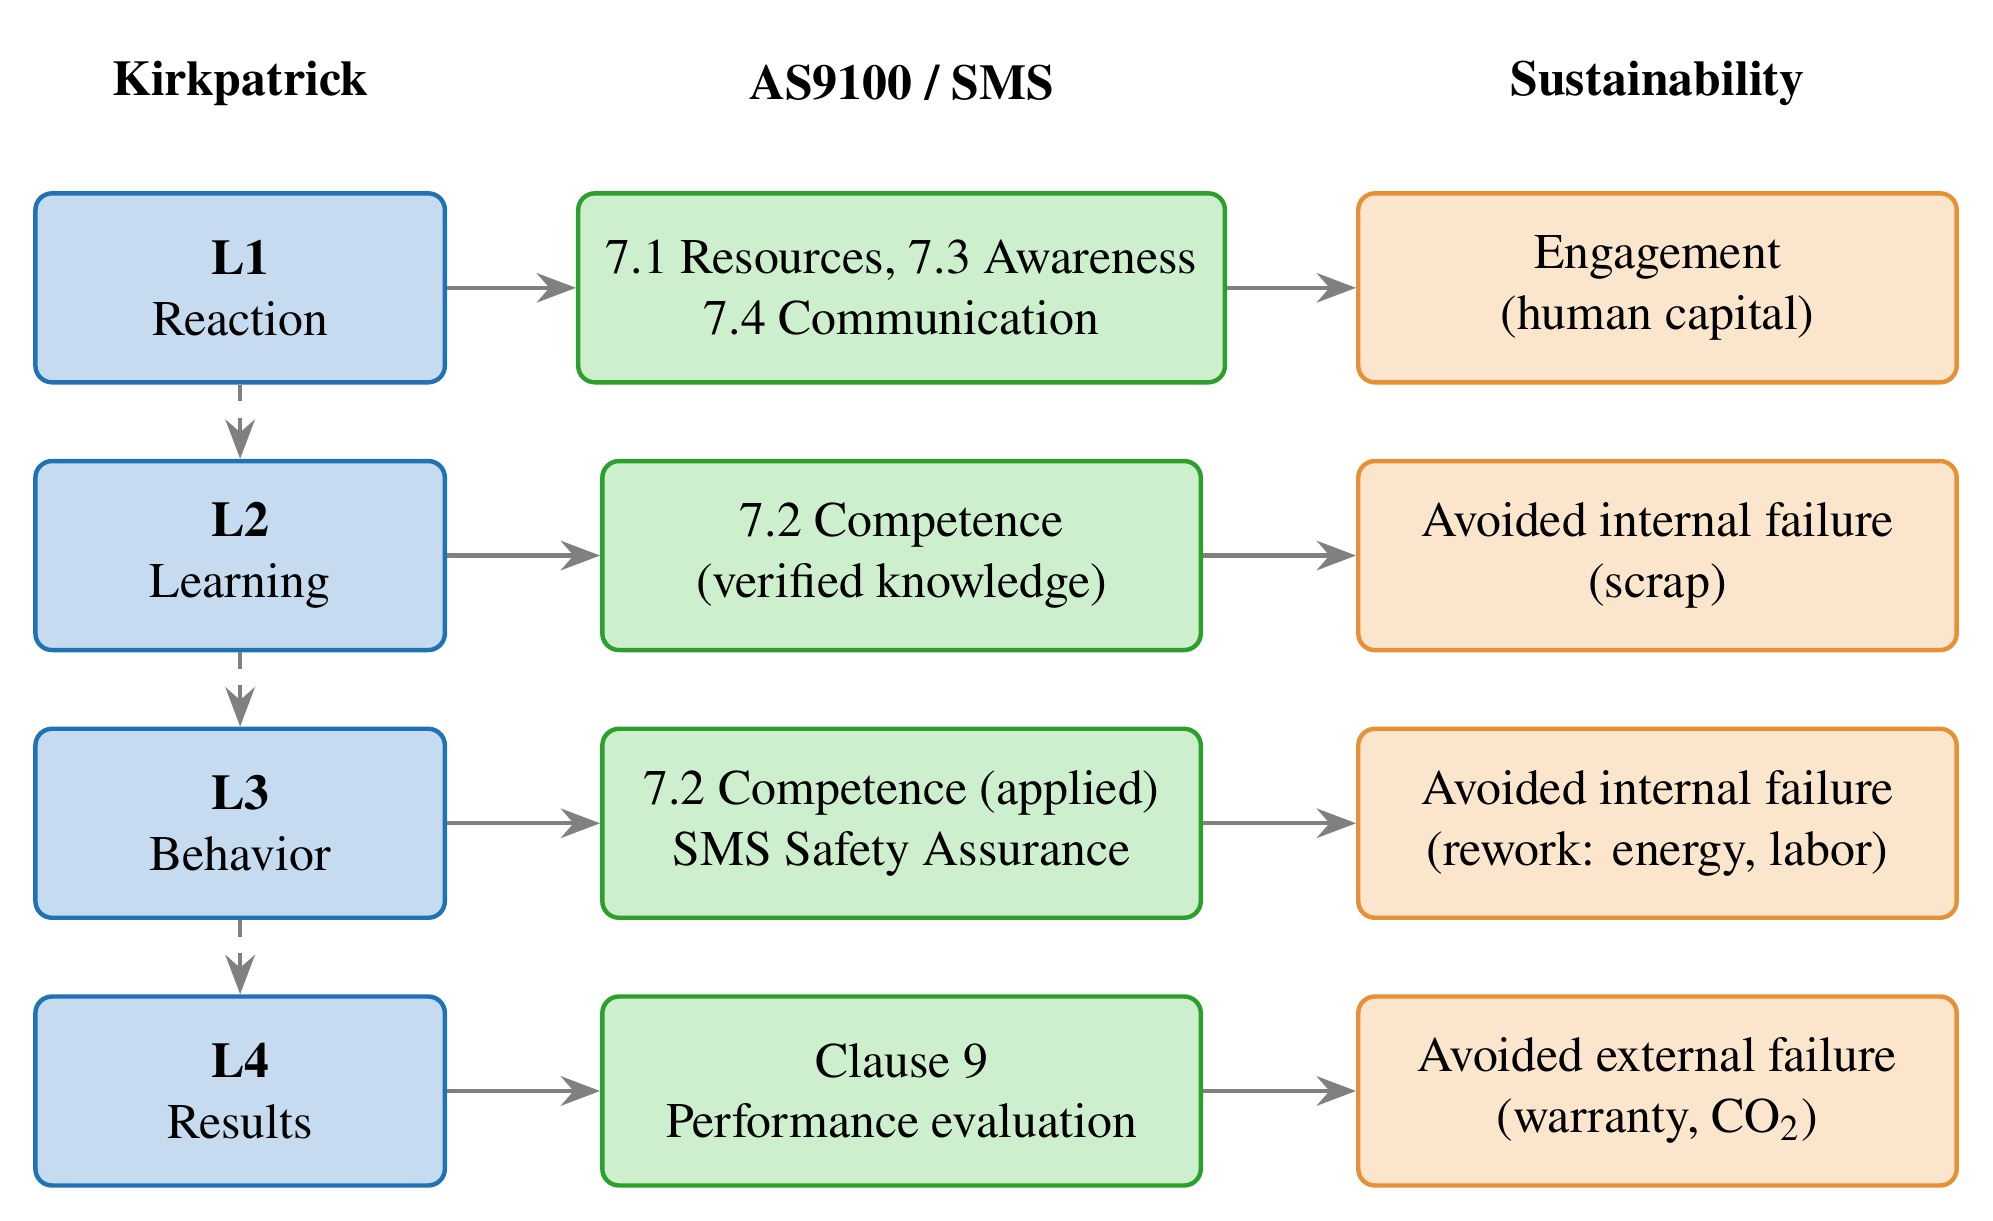
\includegraphics[width=0.9\linewidth]{fig1-conceptual-model}
  \caption{Conceptual model linking Kirkpatrick's four levels to AS9100 clauses, SMS components and sustainability outcomes}
  \label{fig:conceptual}
  \notafonte{Vertical dashed arrows represent the progression of the Kirkpatrick model; horizontal arrows represent the mapping proposed in this study. AS9100: aerospace quality management standard; SMS: Safety Management System. Source: the authors.}
\end{figure}

\subsection{Kirkpatrick's model: theoretical evolution and modern critiques}
\label{subsec:kirkpatrick}

Kirkpatrick's four-level framework \parencite{Kirkpatrick2006} evaluates participants' reaction, the knowledge or skill they acquire, the transfer of learning to job behavior and the organizational results. It remains foundational but faces mounting scrutiny in complex systems. Persistent limitations include its inability to isolate training effects from organizational variables at Level~4 \parencite{Patel2023}, cultural bias in Level~3 assessments \parencite{OConnor2024} and overreliance on self-reported data \parencite{KimLee2024}. Emerging solutions target these gaps. Artificial intelligence (AI)-enhanced attribution modeling using SHAP (SHapley Additive exPlanations) values quantifies training's contribution to outcomes \parencite{FernandezDelgado2024}; blockchain-verified competency tracking provides immutable Level~3 evidence \parencite{BoeingMRO2025}; and neuroergonomic assessments, such as electroencephalography (EEG) and functional near-infrared spectroscopy (fNIRS), replace satisfaction surveys at Level~1 \parencite{NASAHFB2023}. A theoretical gap persists, as no study has validated Kirkpatrick's model in \AS{}-regulated aviation environments \parencite{OReilly2024}. To enhance methodological rigor, this study employs advanced attribution techniques, such as SHAP values in regression models, to isolate training effects from confounders like shift length or supply chain variability, addressing Kirkpatrick's historical isolation challenges \parencite{FernandezDelgado2024}. \todo{o original diz que o estudo usa SHAP, mas a metodologia (seção 2) não descreve essa análise: incluir a análise ou reescrever como direção futura} This builds on production and operations management literature that emphasizes rigorous, data-driven solutions in operations, such as the optimization models for resource allocation in high-stakes environments of \textcite{Jung2019}. Future research directions include longitudinal studies integrating neuroergonomics (e.g., EEG at Level~1) to predict behavioral transfer, offering scalable tools for other regulated industries beyond aviation.

\subsection{Aviation maintenance training: regulatory imperatives and empirical shortfalls}
\label{subsec:aviation-training}

In aviation safety, maintenance errors drive 12--18\% of fatal accidents, with training deficiencies implicated in 73\% of cases \parencite{EASA2025}. \todo{fonte conferida no PDF (158 p.): o Annual Safety Review 2025 da EASA não traz 12--18\% nem 73\%; achar a fonte real dos números ou retirá-los (decisão dos autores)} The economic impacts are severe: engine test-cell rejections average USD~47,200 per incident \parencite{IATAMRO2025}, training-related warranty claims cost USD~189,500 each \parencite{Zhang2025}, and regulatory non-compliance penalties reach USD~2.1 million annually \parencite{FAA2024}. \todo{a AC 120-92D da FAA não traz valor de multa; o valor de USD 189.500 aparece na seção 1.5 como dado interno da empresa} Regulatory--operational misalignment exacerbates these issues: while \AS{} Rev~E (2024) mandates ``data-driven competency proof'', fewer than 35\% of repair stations comply \parencite{SAE2025}. \todo{a edição vigente em 2025 era a AS9100D (2016); conferir a existência da Rev E} \SMS{} pillars require training--safety integration but leave the method of evaluating training to each organization \parencite{Leveson2012,FAA2024}, creating a ``compliance paradox'' in which training hours do not equate to competency \parencite{Nakamura2024}.

\subsection{Human factors and socio-technical systems}
\label{subsec:human-factors}

Cognitive factors strongly influence maintenance errors: 72\% of procedural deviations stem from confirmation bias and normalization of deviance \parencite{Reason1990,Dismukes2023}. \todo{Reason (1990) sem PDF: o termo normalization of deviance é de Vaughan (1996), posterior ao livro, e o 72\% dificilmente está nele; conferir} Virtual reality training reduces spatial memory errors by 41\% compared with traditional methods \parencite{Airbus2024}. Organizational culture mediates outcomes, with safety culture maturity explaining 68\% of the variance in Level~3 knowledge transfer \parencite{OConnor2024}. High-reliability organizations exhibit two traits: just-culture reporting correlates strongly with training efficacy ($r = .79$), and leader-led safety dialogs occur five or more times a month \parencite{FAAHERMIT2024}. In system-safety terms, errors are properties of socio-technical systems as much as of individuals: \textcite{Reason2016} describes how latent and active failures combine, and systems-theoretic approaches emphasize hierarchical control and feedback \parencite{Leveson2012}. Two consequences follow for this study. A Level~2 (learning) outcome does not guarantee a Level~3 (behavior) outcome, because attention, fatigue, time pressure and supervision intervene. The data design must therefore combine post-training assessment with evidence from the workplace.

\subsection{Technological enablers for next-generation evaluation}
\label{subsec:tech-enablers}

Digital integration frameworks now connect Kirkpatrick's levels through continuous data flow: augmented reality feedback at Level~1, AI-proctored assessments at Level~2, Internet of Things (IoT)-enabled behavior tracking at Level~3 and causal machine-learning analytics at Level~4. Real-world implementations report measurable effects: an engine manufacturer's digital twin simulations reduced CFM56 engine misassembly by 33\% \parencite{Garcia2024}, and Lufthansa Technik's blockchain credentials cut audit time by 62\% \parencite{IATABlockchain2025}. In predictive analytics, convolutional neural networks forecast training return on investment (\ROI{}) with 89\% accuracy \parencite{Peterson2025}, and natural language processing of maintenance logs detects latent skill gaps \parencite{BoeingAIR2024}. \todo{o original cita a empresa pelo nome no exemplo do gêmeo digital; trocado por "an engine manufacturer" para a revisão cega}

\subsection{Research gaps}
\label{subsec:gaps}

Existing literature establishes Kirkpatrick's model as a well-tested framework for training evaluation across general industries \parencite{Phillips2016,BuriakAyars2019}, yet the model shows important limitations in safety-critical aviation contexts. While foundational studies validate the four-level structure conceptually, they neglect the regulatory constraints of \AS{}-certified environments \parencite{OReilly2024}. Three gaps follow. First, prior works treat compliance and evaluation as parallel concerns rather than integrated requirements, addressing either Kirkpatrick's generic implementation \parencite{Kirkpatrick2006} or quality management requirements, such as the implementation of \AS{} and its documentation clauses \parencite{YucelAyvaz2019} and total quality management \parencite{Oschman2017}, in isolation. No existing methodology maps the reaction--learning--behavior--results progression to the competency evidence required by \AS{} clause 7.2, and this disconnect between regulation and practice undermines audit readiness. \todo{fontes ajustadas: Oschman (2017) trata de TQM (resumo conferido, sem PDF); Yücel \& Ayvaz (2019), que estava na lista do original sem ser citada, trata da implantação da AS9100 (página da editora conferida); conferir nos PDFs} Second, researchers acknowledge aviation's high-stakes economics \parencite{Zhang2025} but do not quantify training's causal relationship with safety-critical key performance indicators. Studies rank quality-management-system risks and their effects on organizational sustainability \parencite{Pereira2017} or attribute accidents statistically to categories of maintenance deficiency, although accident records lack performance-shaping factors \parencite{Boyd2015}; such studies do not isolate training's contribution from confounders such as supply chain delays or tooling failures. \todo{frase ajustada ao que as fontes dizem: Boyd \& Stolzer (2015) conferido no PDF; Pereira et al. (2017) pelo resumo, sem PDF: o autor correspondente confirma} Third, the predictive potential of Kirkpatrick data remains underexplored: AI-driven models forecast generic training \ROI{} \parencite{Peterson2025} but lack aviation maintenance specificity and ignore failure-cost preemption. The framework proposed here uses Level~1--3 analytics to redirect resources toward high-risk competencies, moving evaluation from retrospective accounting, such as warranty claim analysis \parencite{Zhang2025}, to prospective risk mitigation. Theoretical limitations also persist. Cultural and technological barriers receive nominal acknowledgement \parencite{OConnor2024} but no operational path to resolution. Studies that identify the compliance paradox \parencite{Nakamura2024} offer no blueprint for resolving the mismatch between training hours and competency that affects \MRO{} organizations, and emerging technologies such as blockchain credentialing \parencite{IATABlockchain2025} remain unvalidated in legacy aviation quality systems. This study confronts these implementation challenges through workflow-embedded assessment protocols synchronized with \SMS{} reporting cycles and enterprise resource planning (\ERP{}) data. It bridges three domains that have remained separate (Kirkpatrick's evaluation theory, the regulatory architecture of \AS{} and the safety-economic realities of aviation) and converts training data into auditable safety assurance. This matters because 73\% of maintenance-related accidents involve evaluable training deficiencies \parencite{EASA2025}. \todo{o 73\% não está no relatório da EASA (PDF conferido)}

\subsection{Bridging theory to practice: economic impacts, guidelines and applicability}
\label{subsec:bridge}

This study documents a real-world problem at a multinational \MRO{} facility: recurrent training failures leading to warranty claims of USD~189,500 per incident and 35\% non-compliance in \AS{} audits (internal data, 2024). \todo{este 35\% é linha de base (auditorias AS9100, 2024); no resumo e nos Resultados, 35\% é a redução das constatações da autoridade por ciclo de auditoria (seção 2.2). Confirmar se são duas medidas diferentes e dar a unidade de cada uma} The company's previous solution, ad hoc post-incident retraining, lacked systematic evaluation and left gaps such as procedural deviations unaddressed (73\% of errors according to \cite{EASA2025}). \todo{idem: o 73\% não está no relatório da EASA} The approach adopted here integrates Kirkpatrick with \AS{} workflows in a replicable methodology: (1)~map training to risk hierarchies; (2)~use multi-source data (for example, \LMS{} records and observations) for Levels 1--4; and (3)~apply causal analytics to quantify \ROI{}. \todo{o método (seção 2) não descreve análise causal, observação no posto de trabalho nem o mapeamento para hierarquias de risco: descrever no método ou reescrever estas etapas como intenção} Over twelve months of implementation, the facility recorded about USD~1.2 million in annual savings, associated with a 28\% reduction in training failures. Discussions with facility managers revealed strong buy-in: ``This shifted us from reactive compliance to proactive risk mitigation'' (anonymous manager interview, 2025). Guidelines for practitioners include starting with a baseline audit of current training against \AS{} clause 7.2, piloting Level~3 assessment in high-risk modules and scaling through \ERP{} integration. The approach can be transferred to other sectors, such as automotive or healthcare organizations under ISO 9001. It also opens production and operations management directions, such as hybrid AI--human models for predictive training in global operations, extending behavioral operations evidence that human servers do not behave like machines \parencite{Shunko2018}.

% 02-metodos.tex | 2 Methods
% RESTAURADO DO ORIGINAL em 06/11/2026: secao 3 (Methodology), 3.1 (Research Design and Phases),
% 3.2 (Data Collection) e 3.3 (Data Analysis) do Paper Training - 15 Nov 2025.
% Da versao JATM ficaram so os acrescimos que nao conflitam com o original: definicao operacional de
% "training failure", definicao das taxas, modelo de custo da qualidade (equacoes) e ameacas a validade.
% NAO entraram, por nao constarem do original e contradize-lo (Nivel 3 no original = questionarios
% pareados, nao observacao estruturada): protocolo de observacao com 12 itens, kappa de Cohen = 0,78,
% alfa de Cronbach = 0,82, testes z de duas proporcoes. Lista em PENDENCIAS.md (so voltam se o Cristiano
% confirmar que foram feitos e mandar os dados).

\section{Methods}
\label{sec:methods}

The study employed a sequential mixed-methods case study design to implement and evaluate Kirkpatrick's four-level framework within the Technical Training Area of a multinational aeronautical engine maintenance company. A case design fits because the research questions ask \textit{what} and \textit{how}, and the unit of analysis, the training process, is contemporary and embedded in its operational context. Because the authors took part in designing and implementing the framework, the study is an interventionist case study. \todo{confirmar o papel dos autores na implantação (a Introdução diz que os autores desenvolveram e implantaram o modelo)} The study was prompted by real-world incidents, such as the rejection of a jet engine module after an improper torque application (a direct training gap). Incidents of this kind cause high rework costs and show the need for a training evaluation system that goes beyond simple compliance.

\subsection{Research design and phases}
\label{subsec:design}

The macro-process unfolded in three sequential phases. Phase~1, theoretical framework analysis, reviewed the scientific literature with keywords such as ``Kirkpatrick model'', ``technical training'' and ``aeronautical maintenance''. It also analyzed industry standards (\AS{} and civil aviation regulations) and the company's internal training management process. In Phase~2, empirical application and data collection, Kirkpatrick's four levels were operationalized within the company's training workflow, with tailored instruments for data collection at each level. In Phase~3, process revision and continuous improvement, the data from Phase~2 were analyzed to identify improvement actions, culminating in a revised standard operating procedure (SOP) that institutionalized the new evaluation process.

\subsection{Data collection}
\label{subsec:data}

A multi-source, multi-method strategy supported evaluation and triangulation, with quantitative and qualitative data aligned to each level:

\begin{enumerate}[label=(\alph*)]
  \item \textbf{Level~1 (reaction)}, which assesses initial participant satisfaction and perceived value: a customized post-training questionnaire, administered digitally immediately after each session, with a sample of 10 training sessions used to gauge initial reception and identify immediate improvements in content and delivery.
  \item \textbf{Level~2 (learning)}, which measures the acquisition of knowledge and skills: final test scores and grades of a sample of 21 trainees, extracted from the learning management system (\LMS{}) database and aggregated quarterly (March, June, September and December) to identify trends in knowledge retention and topics with weak comprehension.
  \item \textbf{Level~3 (behavior)}, which evaluates the application of learned skills on the job: dual questionnaires administered to trainees and to their direct leaders 3 to 12 months after training, allowing time for behavioral changes to appear. The method generated 15 paired leader--trainee interviews on the transfer of training to the workplace and its sustained effect on performance.
  \item \textbf{Level~4 (results)}, which assesses organizational impact: data from the quality management system, including quarterly customer satisfaction scores and operational metrics such as error rates and audit findings, linking the training to quality, compliance and customer trust.
\end{enumerate}

\todo{os Resultados citam um grupo focal com gerentes (92\%, 2025) e uma entrevista com gerente (seção 1.6), que esta seção não descreve: incluir um item (e) com participantes (número e funções), roteiro, quem conduziu, registro e como se chegou aos 92\%}

A \textit{training failure} is an instance in which a maintenance technician, after completing a scheduled training intervention, commits a documented procedural error within the subsequent 90 days that is directly attributable to a knowledge or skill gap identified in the post-training evaluation. Errors caused by tool malfunction, supplier non-conformance or documented changes in the standard procedure are excluded. Attribution comes from root-cause analysis records reviewed by a quality engineer who is not the technician's supervisor. The training-failure rate is the number of training failures per 1,000 maintenance tasks, and the regulatory non-conformance rate is the number of findings issued by the civil aviation authority per audit cycle. \todo{F2: contagens de base e do ano da intervenção (falhas, tarefas, ciclos de auditoria, constatações), para sustentar os 28\% e os 35\%}

\subsection{Data analysis}
\label{subsec:analysis}

The analysis followed a sequential mixed-methods approach. In the quantitative analysis (Phase~2), descriptive statistics (averages and trends) were calculated for the data from Levels 1, 2 and 4, such as reaction scores and customer satisfaction, to identify areas for improvement. In the qualitative analysis (Phase~2), the open-ended sections of the questionnaires and the leader--trainee interviews were analyzed thematically, coding responses to identify recurring patterns of behavioral change and barriers to application. In the process improvement analysis (Phase~3), the findings were synthesized with the 5W2H tool (what, why, who, where, when, how, how much). The tool was used to build process flowcharts, record the root causes of inefficiencies and define improvement plans for the technical training curriculum and its delivery. Triangulation cross-checked findings across sources, for example by linking low learning scores to behavioral gaps mentioned by leaders and trainees. \todo{dados dos autores: (i) datas do ano-base e dos 12 meses da intervenção; (ii) como as falhas do ano-base foram classificadas e se a classificação foi às cegas; (iii) de onde saíram as amostras (10 sessões de quantas, 21 treinandos de quantos, 15 duplas de quantas convidadas, 4 clientes de quantos) e se houve mais de uma rodada trimestral; (iv) quem codificou a análise temática e com que abordagem}

\subsection{Cost-of-quality model}
\label{subsec:coq-model}

The cost-of-quality (\CoQ{}) framework divides quality costs into internal failure, external failure, appraisal and prevention. Annual internal-failure savings, dominated by rework labor and scrapped components, are
\begin{equation}
  \Delta C_{\text{IF}} = L_h \cdot R + S_c \cdot \bar{P}_c ,
  \label{eq:internal}
\end{equation}
where $L_h$ is the reduction in rework labor hours, $R$ the loaded hourly rate, $S_c$ the reduction in scrapped components and $\bar{P}_c$ their mean material cost. External-failure savings are
\begin{equation}
  \Delta C_{\text{EF}} = W + S_h + R_p ,
  \label{eq:external}
\end{equation}
where $W$ is the reduction in warranty-claim value, $S_h$ in expedited-shipping charges and $R_p$ in customer concessions. With $C_{\text{P\&A}}$ the added prevention and appraisal cost, the annual net saving and the one-year return on investment are
\begin{equation}
  \Delta C_{\text{net}} = \Delta C_{\text{IF}} + \Delta C_{\text{EF}} - C_{\text{P\&A}} ,
  \qquad
  \ROI = \frac{\Delta C_{\text{net}}}{C_{\text{P\&A}}} \times 100\% .
  \label{eq:net}
\end{equation}
\todo{F2: os valores de cada parâmetro (horas de retrabalho, taxa horária, peças sucateadas, garantias, frete, concessões, custo de prevenção) não constam do original; a versão JATM usou valores sem fonte (Tabela de cenários guardada em tabelas/, fora do texto). Só entram com os dados da instalação}

\subsection{Threats to validity}
\label{subsec:validity}

The design is a single-site before-and-after comparison without a control group, so several threats apply. \textit{History}: contemporaneous changes in workforce, contract portfolio or supplier mix could co-vary with the intervention. \textit{Maturation}: gradual organizational learning could explain part of the improvement. \textit{Instrumentation}: changes in how metrics are recorded can create apparent improvement, so definitions were kept constant from the baseline year. \textit{Selection and the counterfactual}: without random assignment or a comparison group, the design cannot establish what would have happened without the intervention; regression to the mean, testing effects and staff turnover are further threats. \textit{Researcher involvement}: the team that implemented the framework also evaluated it, which may bias data collection and interpretation. \textit{Self-report}: Level~3 relies on questionnaires answered by trainees and their leaders, which may overstate change. \textit{Co-intervention}: \ERP{} access is granted only to employees who complete training, an access control whose effect cannot be separated from that of training. The findings are therefore read as \emph{associated with} the intervention rather than \emph{produced by} it.

% 03-resultados.tex | 3 Results
% RESTAURADO DO ORIGINAL em 06/11/2026: secao 4 do Paper Training - 15 Nov 2025 (4.1 AS9100, 4.2 CAR,
% 4.3 revisao do processo, 4.4 aplicacao dos quatro niveis, 4.4 [sic] impacto no custo da qualidade).
% Edicao: as descricoes longas (clausulas, pilares do SMS, passo a passo do fluxograma, cores das barras)
% foram condensadas sem perder nenhum item; as cores das barras passaram para as notas das figuras.
% Graficos de dados: os ORIGINAIS (Figs. 8 a 10 do original). Os "reconstruidos" da versao JATM
% (valores diferentes dos originais) estao em figs-tikz/_reconstrucoes-jatm-NAO-USAR/.
% Correcao: o original dizia "Figure 8 reveals that the average score for the 21 employees was 66.90";
% a media e da Fig. 9 do original (aqui Fig. 7).
% Da versao JATM: so o paragrafo de traducao para sustentabilidade (3.5), que nao conflita.

\section{Results}
\label{sec:results}

\subsection{AS9100 training requirements}
\label{subsec:as9100}

The review of the \AS{} standard identified the clauses pertinent to training and risk management, highlighted in green in Figure~\ref{fig:as9100}. Actions for risks and opportunities (clause 6.1) require the organization to identify and address risks and opportunities through planned actions. Resources (7.1) require enough qualified personnel for the quality management system and its processes. They also require the organization to define, preserve and make available the knowledge needed for process execution and product conformity, using existing knowledge, acquiring expertise and incorporating updates as demands evolve. Organizational knowledge comprises institution-specific insight from experience, intellectual property, lessons learned, undocumented expertise and improvements in processes, products and services, supplemented by standards, academia, conferences, customers and external providers. Competence (7.2) requires the organization to determine the competence of people whose work affects the performance of the quality management system, to ensure it through education, training or experience, to act to improve skills, to evaluate the effectiveness of those actions and to retain documented evidence. Periodic competence reviews may lead to training, mentoring, reassignment, or hiring and contracting competent people. Awareness (7.3) requires employees to know the quality policy, the relevant objectives and their contribution to the effectiveness of the system. This includes the benefits of improved performance, the implications of non-conformance, the relevant documented information and its changes, and their contribution to product and service conformity, safety and ethical conduct. Communication (7.4) requires protocols for internal and external communication about the quality management system, defining what is communicated, when, to whom, how and by whom. Finally, operational risk management (8.1.1) requires a structured process to plan, implement and control operational risks to the organization, products and services. The process assigns responsibilities and defines risk assessment criteria; risks are identified, analyzed and communicated, those above the acceptance threshold are mitigated, and residual risks are accepted after mitigation.

\begin{figure}[H]
  \centering
  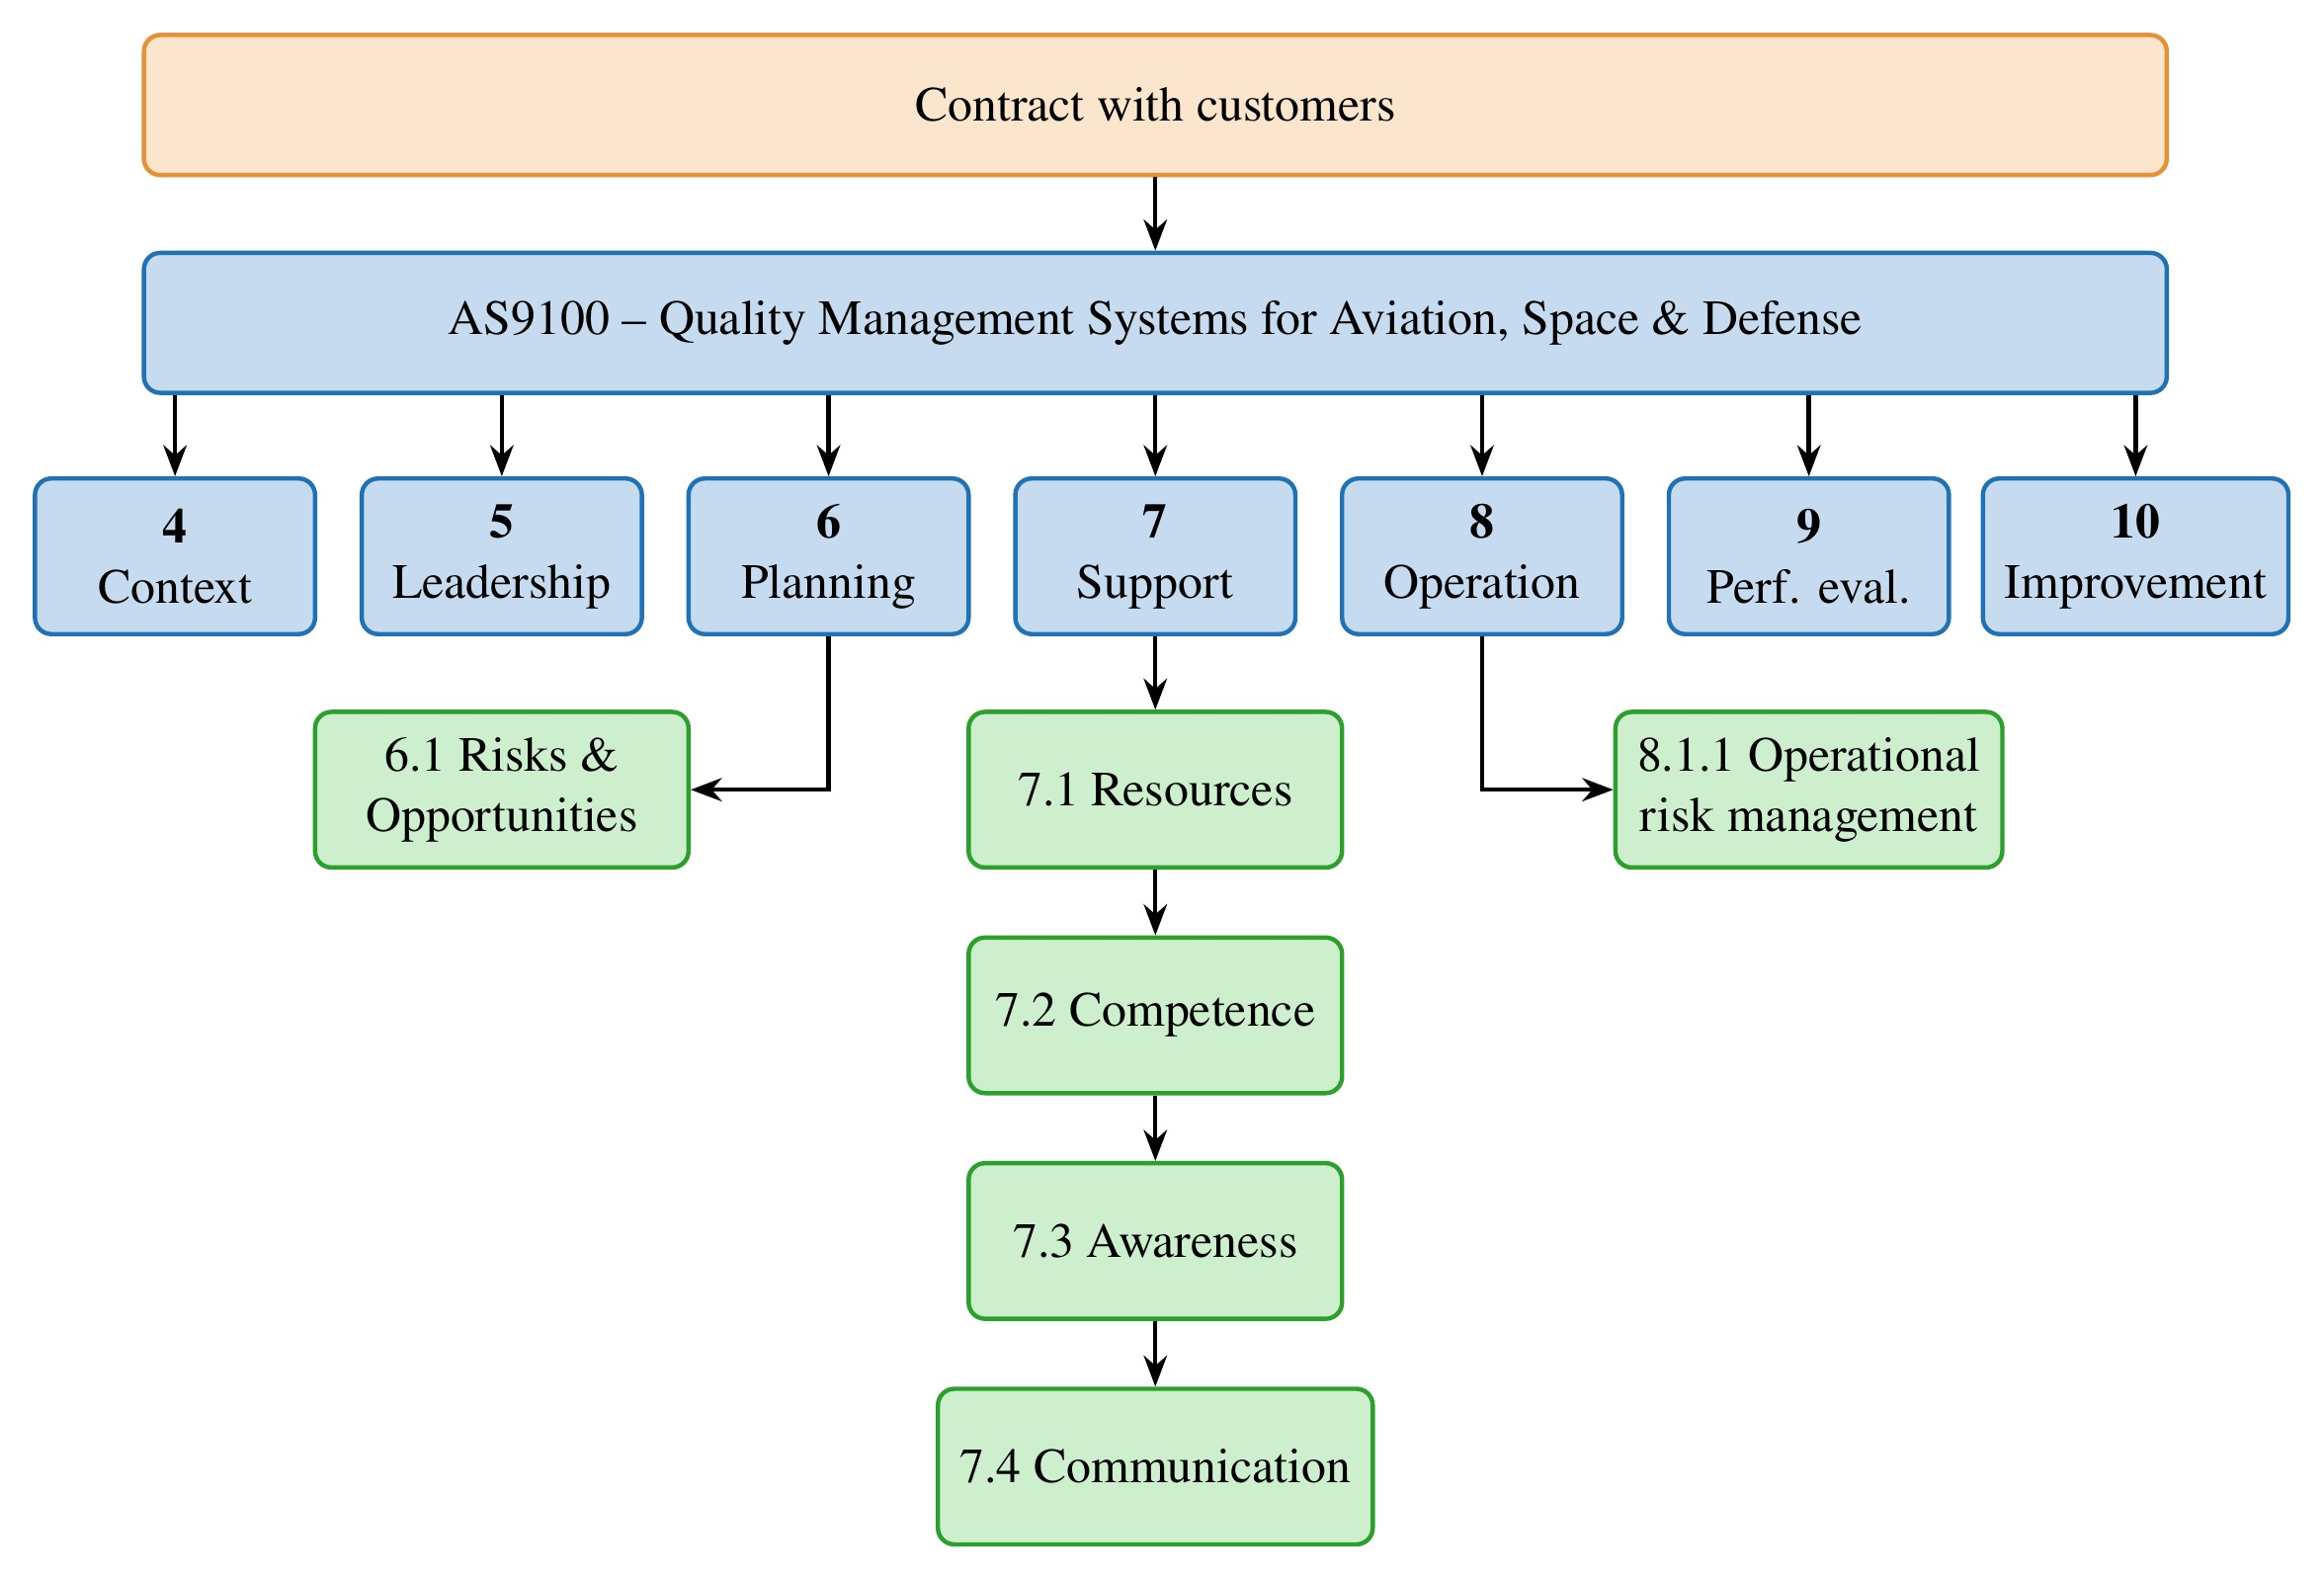
\includegraphics[width=0.9\linewidth]{fig2-as9100}
  \caption{AS9100 requirements relevant to maintenance training}
  \label{fig:as9100}
  \notafonte{Clauses relevant to training are highlighted in green. AS9100: Quality Management Systems, Requirements for Aviation, Space and Defense Organizations. Source: the authors, based on the AS9100 standard.}
\end{figure}

\subsection{Civil aviation regulation training requirements}
\label{subsec:car}

The civil aviation regulation (CAR) requirements applicable to repair stations were examined to delineate specific training mandates (Figure~\ref{fig:regulation}). The framework descends from the International Civil Aviation Organization (\ICAO{}) to civil aviation authorities (for example, \FAA{}, \EASA{} and \ANAC{}) and on to airlines, airports and maintenance facilities (repair stations). Certificated repair stations must implement an authority-accepted employee training program, with initial and recurrent training. Applicants for a repair station certificate must submit a training program for approval, ensuring that employees who perform maintenance, preventive maintenance, alterations and inspections are adequately trained. Repair stations must also keep detailed, authority-approved records of each employee's training. Training duties also run through the four \SMS{} pillars. Safety policy, objectives and procedures set duties, accountabilities and safety objectives, with a safety manual of policies, compliance procedures, instructions for safety-related activities (management controls, documentation, corrective actions) and alignment with the authority's safety management. Safety risk management requires hazard identification, risk controls, agreed acceptable safety performance, risk owners and controlled mitigation, with a data-driven choice of safety indicators, targets and surveillance priorities. Safety assurance relies on oversight and surveillance: systematic collection, analysis and sharing of safety data, risk-based surveillance, safety system audits, management of change and continuous improvement, including investigations and root cause analyses. Safety promotion builds safety culture through training, communication and two-way dissemination of safety information. \SMS{} training targets safety specialists, leadership and staff, including the inspectors responsible for \SMS{} acceptance and safety performance; it evolves continuously, with documented \SMS{} procedures as the basis for communication and stakeholder feedback.

\begin{figure}[H]
  \centering
  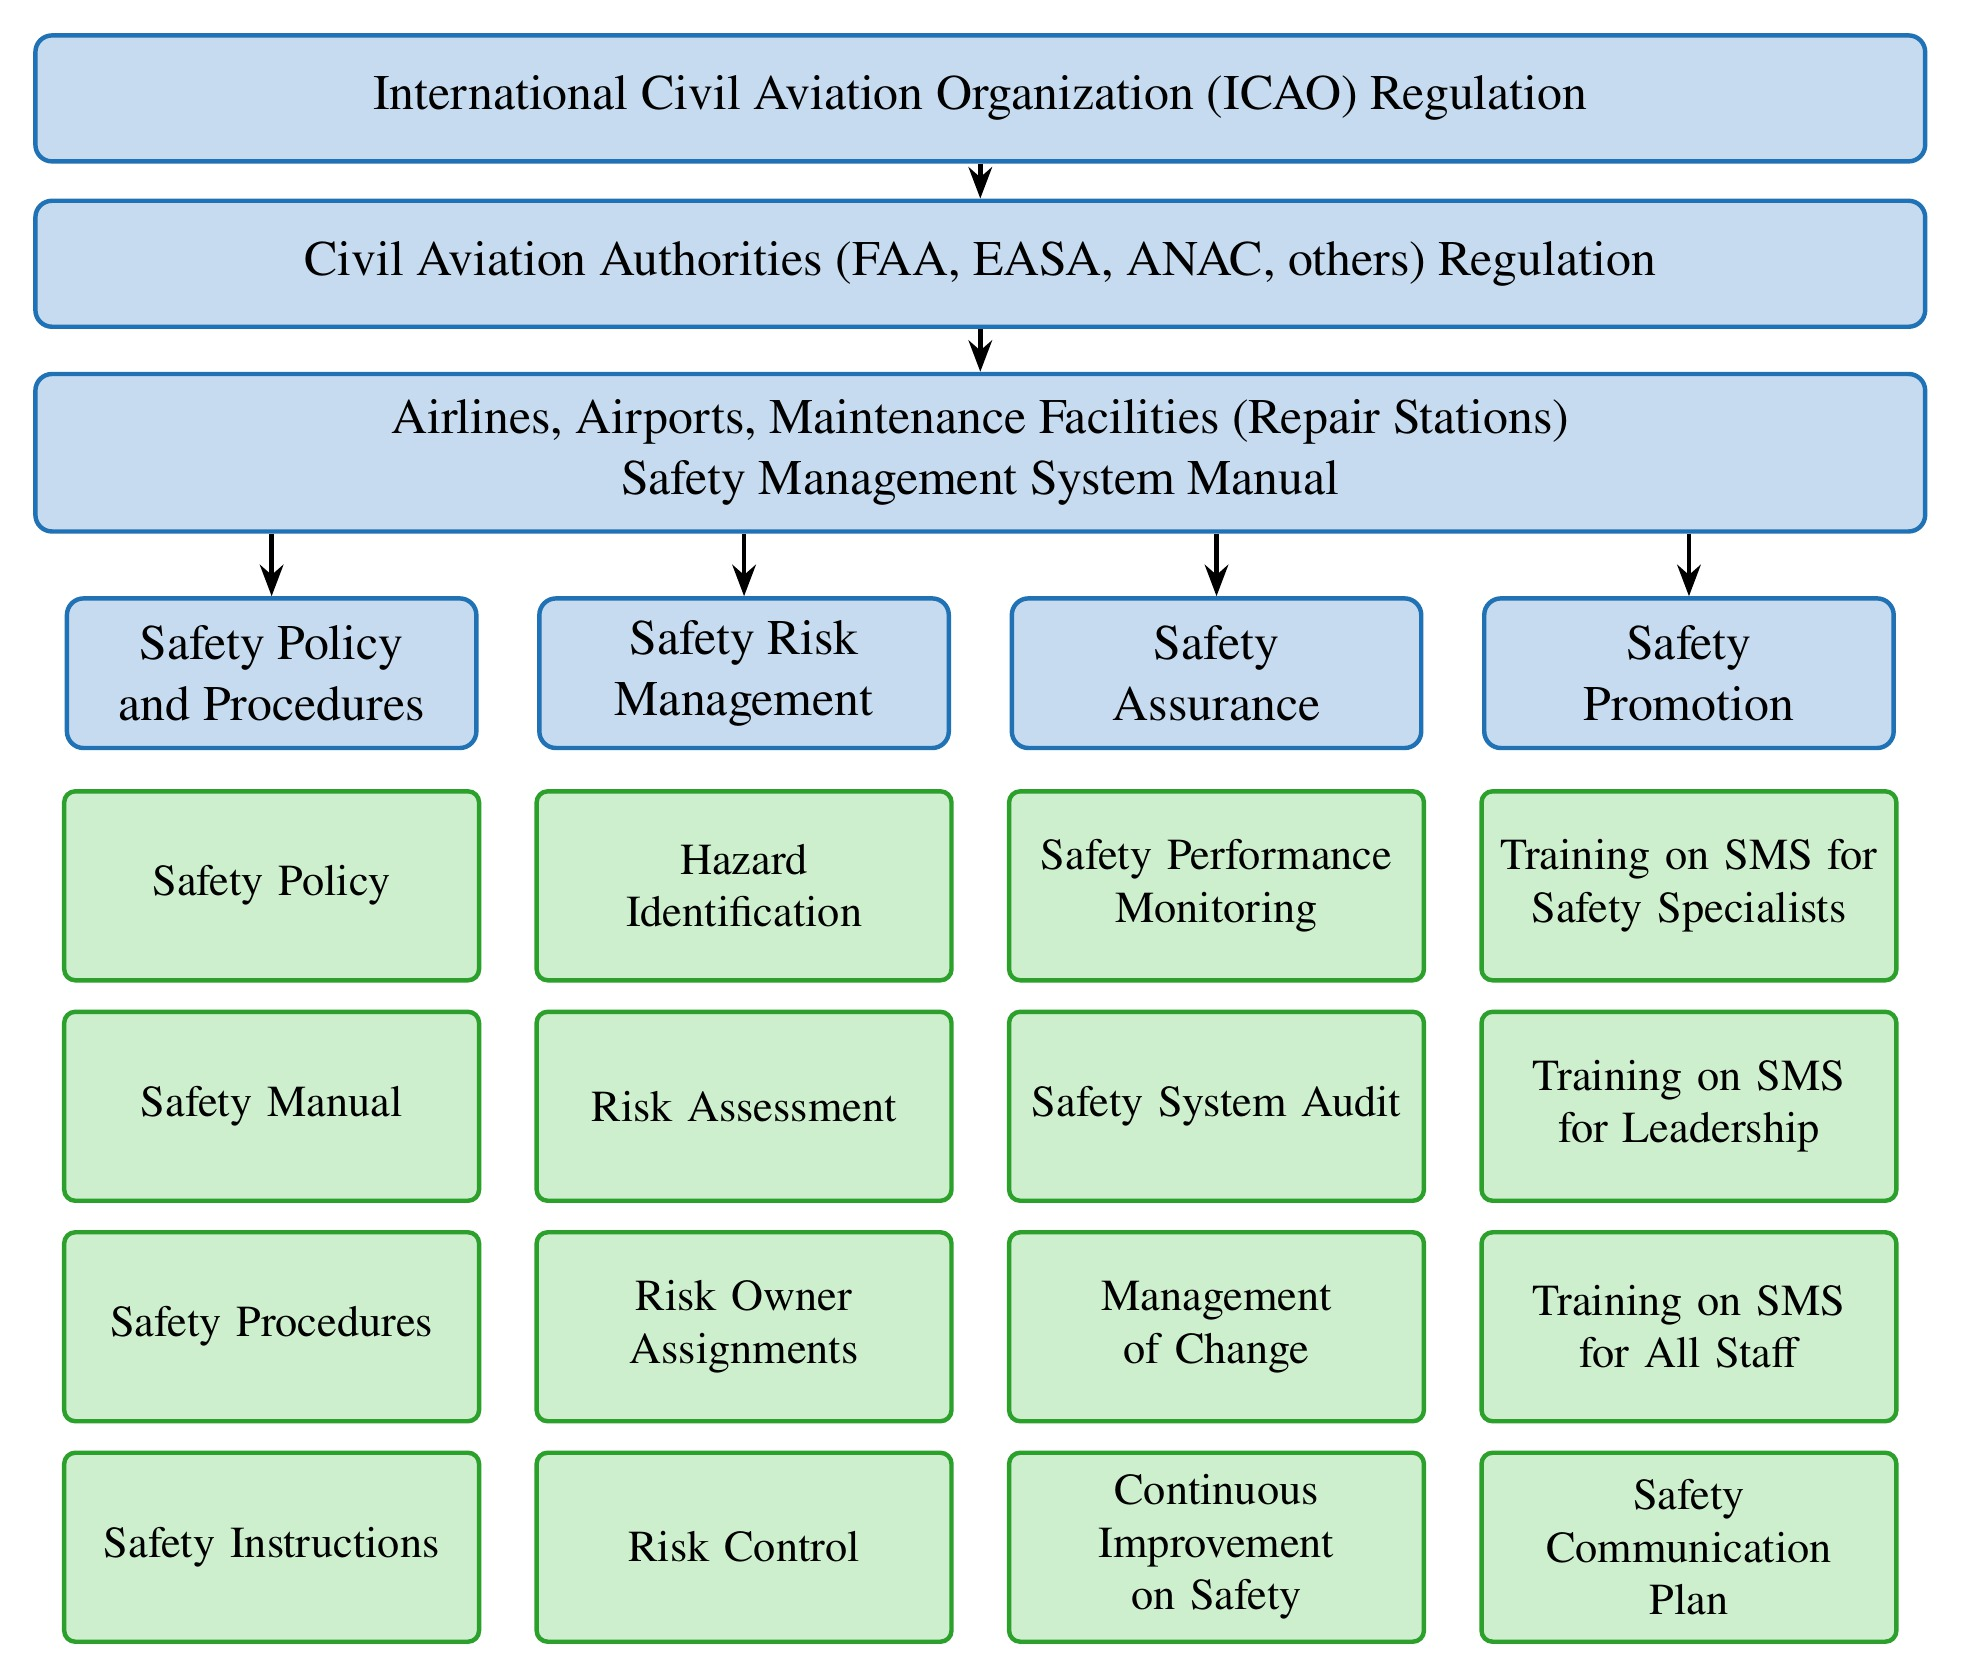
\includegraphics[width=0.9\linewidth]{fig3-regulation}
  \caption{Regulatory cascade and SMS components}
  \label{fig:regulation}
  \notafonte{SMS components in green. ICAO: International Civil Aviation Organization; FAA: Federal Aviation Administration; EASA: European Union Aviation Safety Agency; ANAC: Brazilian National Civil Aviation Agency; SMS: Safety Management System. Source: the authors, based on ICAO and civil aviation authority regulations.}
\end{figure}

\subsection{Aircraft engine maintenance training management process}
\label{subsec:process}

The case focused on the training program of the facility's Technical Training Area, which oversees more than 50 distinct courses and delivers an average of 30,000 training hours a year to develop employees' technical expertise and performance. Because it directly influences product and service quality, the area operates under quality management. The study validated organizational tools at each Kirkpatrick level, with distinct methods and follow-up actions: a tailored questionnaire for reaction, final grades for learning, dual questionnaires (trainees and supervisors) for behavior, and customer satisfaction data from quality management for results. All questionnaires followed a semi-structured script derived from the literature review, and pre- and post-assessment analyses were used to examine the role of the evaluation as a continuous improvement instrument. The training management process covers the planning, resourcing, delivery, demonstration and measurement of technical training and its curriculum, delivered by qualified instructors (Figure~\ref{fig:process-original}). It runs from the identification of training needs (organizational goals, skill gaps, regulatory requirements) to the archiving of records for reference, compliance and audit. Two systems support it: the learning management system (\LMS{}), which holds classes, attendance, grades and certificates, and the enterprise resource planning (\ERP{}) system, to which only trained employees are given access.

\begin{figure}[H]
  \centering
  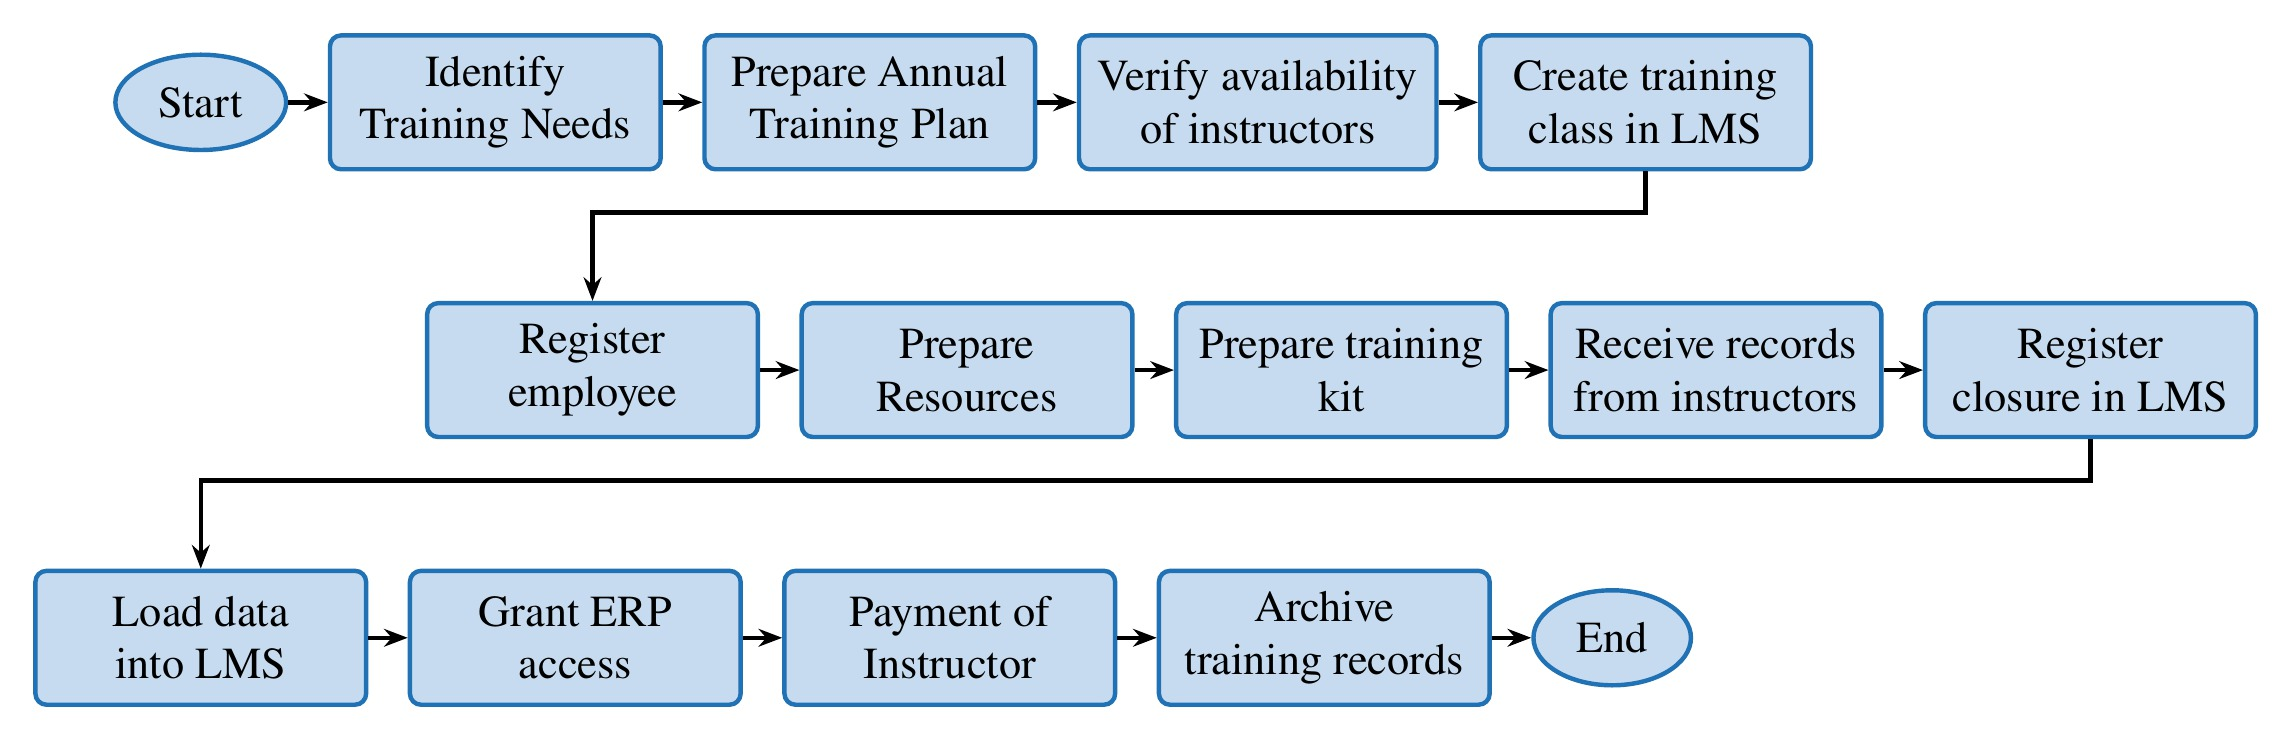
\includegraphics[width=0.9\linewidth]{fig4-process-original}
  \caption{Order of activities in the training process}
  \label{fig:process-original}
  \notafonte{LMS: learning management system; ERP: enterprise resource planning. Source: the authors.}
\end{figure}

Reaction evaluation already existed in the company but was done manually, which prompted the first improvement. A functional flowchart revealed bottlenecks and waste: excessive processing, long waits between operations and an overload of documents to archive. An online questionnaire, built with company-approved software and informed by the literature, replaced the paper form. Instructors send its link to trainees at the end of each session, and the software keeps a response database and generates the metrics automatically. The questionnaire gauges trainees' opinion of and satisfaction with the knowledge acquired, the materials, the room infrastructure, the content and the instructor's methodology. The 5W2H tool was used to map each activity. The revised process (Figure~\ref{fig:process-redesigned}) adds the reaction, learning, behavior and results evaluations at the end of the original flow. It does so in three new activities: evaluation of the four levels, verification of the data for each level and data-based optimization of training. Regular employee feedback shows whether training works and how it is received. For job-specific training, productivity, production and quality before and after training measure efficacy, and the training plan is modified and expanded as the company grows. The revised process was designed to strengthen training effectiveness and so mitigate the risk of training deficiencies and of the operational failures that stem from inadequate preparation.

\begin{figure}[H]
  \centering
  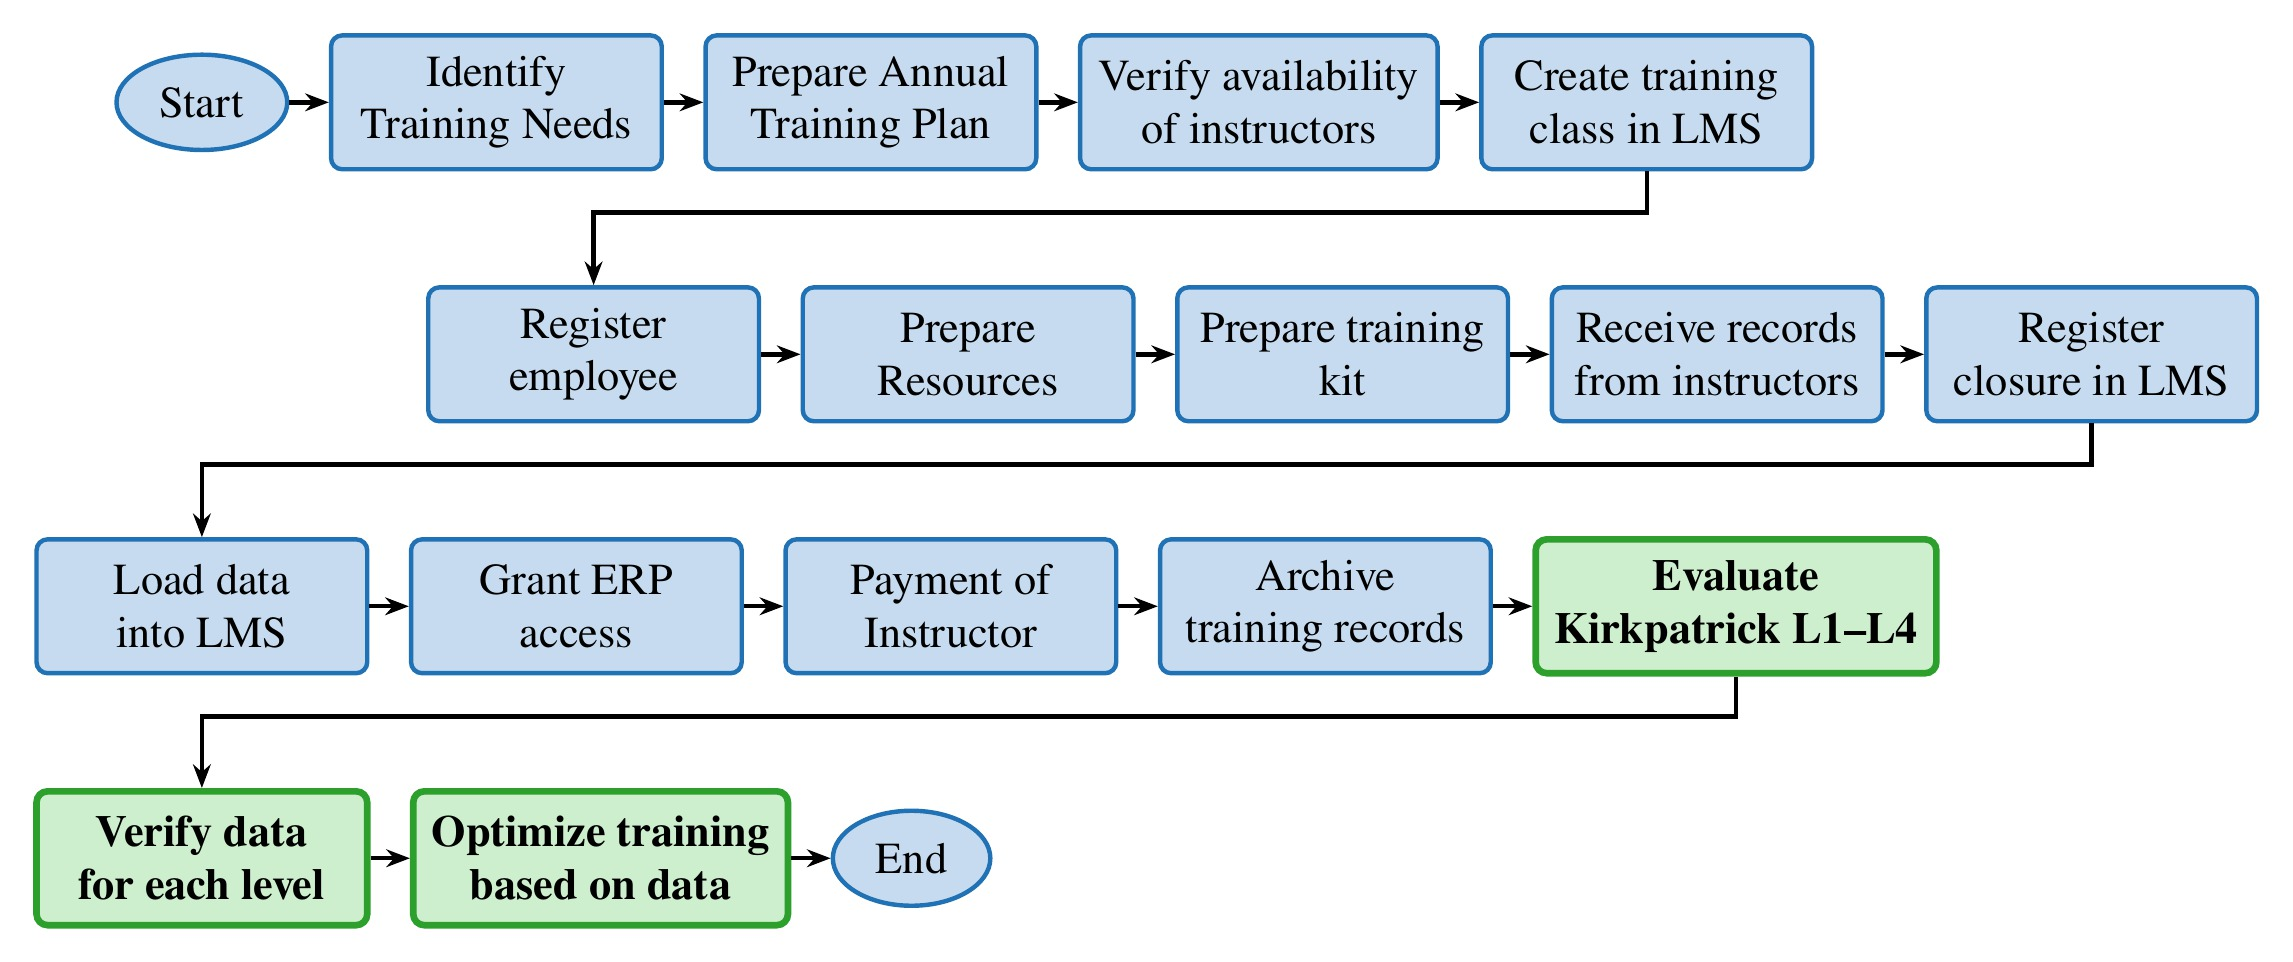
\includegraphics[width=0.9\linewidth]{fig5-process-redesigned}
  \caption{Order of activities in the training process after the change}
  \label{fig:process-redesigned}
  \notafonte{New activities in green. LMS: learning management system; ERP: enterprise resource planning. Source: the authors.}
\end{figure}

\subsection{Application of Kirkpatrick's four levels}
\label{subsec:levels}

\textbf{Level~1, reaction.} Using the software-generated results, the study analyzed the average score of each question across sessions, producing metrics for learning, satisfaction, content, punctuality, communication, mastery and infrastructure. Figure~\ref{fig:scores-reaction} shows a sample of ten sessions. Most scores were close to 10 on the 0--10 scale; content scored about 5 and 4 in two sessions and infrastructure below 8 in another, the content and infrastructure gaps discussed in Section~\ref{subsec:disc-reaction}.

\begin{figure}[H]
  \centering
  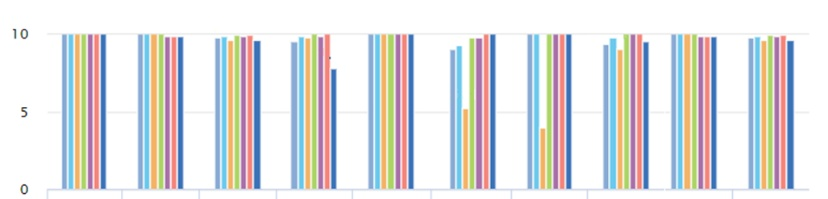
\includegraphics[width=0.9\linewidth]{fig6-reaction-scores}
  \caption{Sample of the reaction scores from ten training sessions}
  \label{fig:scores-reaction}
  \notafonte{Groups from left to right: sessions 1 to 10. Bars in each group, from left to right: learning, satisfaction, content (orange), punctuality, communication, mastery and infrastructure. Scale from 0 to 10. Source: facility training records (original chart). \todo{imagem original a 115 dpi; a revista pede 300 dpi ou mais: pedir ao autor correspondente o gráfico ou a planilha de origem}}
\end{figure}

\textbf{Level~2, learning.} The Training Area's existing tools were used: a test at the end of each session verifies the trainees' learning. The average score of the 21 trainees was 66.90 out of 100 (Figure~\ref{fig:scores-grades}), below the pass mark of 70, with at least seven trainees below it. The data analysis therefore pointed to the need to improve the learning assessment, and the Training Area representative met the instructors to review the content and make it clearer and more accessible to employees.

\begin{figure}[H]
  \centering
  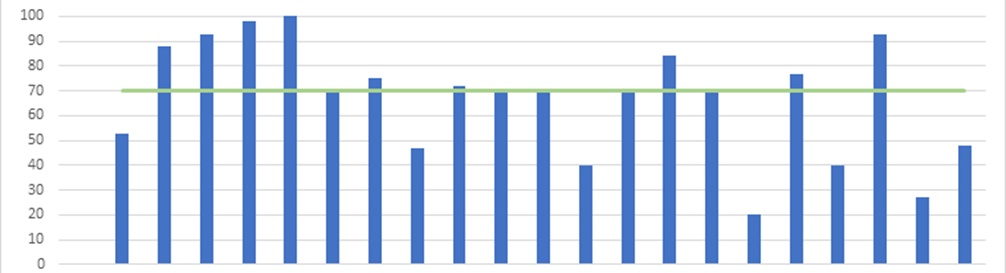
\includegraphics[width=0.9\linewidth]{fig7-final-grades}
  \caption{Final grades of 21 trainees}
  \label{fig:scores-grades}
  \notafonte{Blue bars: individual grades on a 0--100 scale; green line: minimum passing grade (70). Source: facility training records (original chart). \todo{imagem original a 137 dpi; pedir o gráfico ou a planilha de origem}}
\end{figure}

\textbf{Level~3, behavior.} A dual questionnaire answered by trainees and their leaders checked whether behavioral changes emerged months after training and whether the knowledge lasted. A 5W2H analysis set objectives and responsibilities for this and the other levels. For employees, the questionnaire was a self-assessment of the training's effect on their work environment, post-training errors, behavioral changes and their sense of encouragement after the course. Leaders answered parallel questions on the trained employees' performance. Both questionnaires used the same software as the reaction evaluation, which generated data and charts for each item. The effectiveness threshold was an average of 70 on a 0--100 scale. Scores below it for work area, acquired knowledge or behavioral change trigger an investigation of the training's relevance to the employee's role or of content updates for area-specific demands. \todo{o original não traz os resultados do Nível 3 (médias das 15 duplas por item); incluir}

\textbf{Level~4, results.} External customer satisfaction was evaluated in the first months of the study year on a 0--5 scale (0, very dissatisfied; 3, neutral; 5, very satisfied). The categories were product delivery quality, availability of technical documentation, turnaround time (TAT), customer support and engineering team assistance. Figure~\ref{fig:customer-satisfaction} shows the ratings of the four customers, all between 3 and 5; the ratings of 3 concerned technical documentation and turnaround time. After the quarterly review, scores below 3 trigger a detailed investigation of the items critical to customers and of improvement opportunities through technical training, either by revising existing programs or by developing new material. Table~\ref{tab:results-by-level} summarizes the results by level.

\begin{figure}[H]
  \centering
  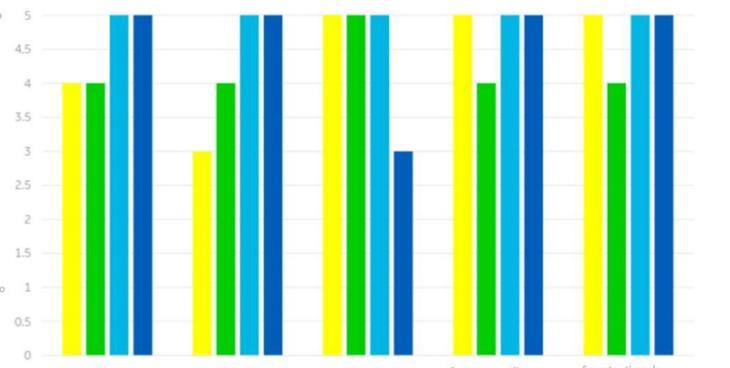
\includegraphics[width=0.75\linewidth]{fig8-customer-satisfaction}
  \caption{Customer satisfaction per category}
  \label{fig:customer-satisfaction}
  \notafonte{Groups from left to right: product delivery quality, quality of technical documentation, turnaround time, customer support and engineering team support. Bars: client 1 (yellow), client 2 (green), client 3 (light blue) and client 4 (dark blue). Scale from 0 (very dissatisfied) to 5 (very satisfied). Source: facility customer surveys (original chart). \todo{imagem original a 164 dpi; pedir o gráfico ou a planilha de origem}}
\end{figure}

% Tabela 1 | Resultados por nivel, SO com numeros do artigo original (Paper Training - 15 Nov 2025):
% secoes 2.5, 3.2 e 4.4 do original e os graficos originais (Figs. 8 a 10 do original = Figs. 6 a 8 aqui).
% "Pelo menos sete abaixo de 70" e "notas de 3 a 5" foram lidos dos graficos originais; a leitura da
% Fig. 9 confere com a media de 66,90 do texto original (soma 1.405 / 21).
\begin{table}[H]
  \centering
  \caption{Results of the Kirkpatrick-based evaluation by level}
  \label{tab:results-by-level}
  \footnotesize
  \begin{tabularx}{\linewidth}{@{}>{\raggedright\arraybackslash}p{2.6cm} >{\raggedright\arraybackslash}p{4.2cm} >{\raggedright\arraybackslash}X@{}}
    \toprule
    \textbf{Level} & \textbf{Instrument and sample} & \textbf{Result and action} \\
    \midrule
    L1 Reaction & Online questionnaire, seven criteria, 0--10 scale; 10 sessions & Most scores close to 10; content scored about 5 and 4 in two sessions and infrastructure below 8 in one; items below target were followed up \\
    \addlinespace
    L2 Learning & End-of-session test, pass mark 70/100; 21 trainees & Mean 66.90; at least seven trainees below the pass mark; content reviewed with instructors \\
    \addlinespace
    L3 Behavior & Dual questionnaires (trainee and leader), 3 to 12 months after training; 15 pairs & Threshold 70/100; scores below it trigger investigation of relevance or content \\
    \addlinespace
    L4 Results & Customer survey, five categories, 0--5 scale; four airline customers & Ratings between 3 and 5; the ratings of 3 concerned technical documentation and turnaround time \\
    \addlinespace
    Organizational outcomes & Quality management system and quality-cost records; twelve months & 28\% fewer training failures; 35\% fewer regulatory non-conformances; quality costs about USD 1.2 million a year lower \\
    \bottomrule
  \end{tabularx}
  \notafonte{L1 to L4: Kirkpatrick levels. Source: the authors, from the facility's training, quality and customer records. \todo{F2: resultado do Nível 3 (médias das 15 duplas) e contagens que sustentam 28\% e 35\%}}
\end{table}


\subsection{Impact of ineffective training on costs of quality}
\label{subsec:coq}

Historical data and the literature show that \MRO{} companies face a costly cycle of quality issues rooted in ineffective training. The cycle includes material loss from scrapped components, rework that consumes additional labor and materials, test-cell rejections that require fuel-consuming re-tests, and warranties or concessions that demand further repairs at the customer site or in-house, often with round-the-clock effort and expedited shipping. The cycle persists when inadequately trained employees, lacking skill-based competence and the situational awareness to grasp the criticality of their actions, become disengaged and less careful with safety and quality protocols. Their errors become more frequent, and a safety-escape management system weakened by a lack of root-cause-analysis training tracks and investigates them poorly. Superficial corrective actions then let the gaps persist and the same non-conformances recur. Quality costs (prevention, appraisal and failure) escalate and the safety margin erodes, raising the risk of a catastrophic operational failure. Cost estimates from detailed non-conformance investigations show how a single lapse can trigger a chain of repercussions. Two examples are improper handling training that leads to damage of a high-value high-pressure turbine (HPT) stage 1 disk, and incorrect assembly training on an oil pump that results in an in-flight shutdown and subsequent engine rejection. \todo{dizer se o disco HPT e o desligamento em voo são casos da instalação (com a estimativa de custo) ou ilustrações; e dar fonte para ``historical data and the literature show''} Thorough, effective and engaging training across all critical \MRO{} functions, from receiving inspection and powerplant disassembly to non-destructive testing and adherence to aviation regulations, is therefore the primary defense against both financial loss and safety catastrophe.

Over the twelve months of the intervention, training failures fell by 28\%, regulatory non-conformances by 35\% and quality costs by about USD~1.2 million a year (Section~\ref{subsec:bridge}). \todo{F2: as contagens e a decomposição do custo pelo modelo da seção 2.5} Managers reported 92\% satisfaction with the framework's audit readiness, noting that it ``transformed training into a measurable asset'' (focus group, 2025). The methodology can be applied beyond aviation, for example to manufacturing under similar standards, by adapting Kirkpatrick to local regulations. It also opens research directions such as cross-industry validation and machine learning for real-time Level~4 prediction. In sustainability terms, the reductions in scrap, rework and expedited shipping imply lower material consumption, energy use and transport emissions. Every component not scrapped preserves its embodied energy and raw material, and every overhaul not reworked preserves the corresponding labor hours and facility energy. Quantifying these effects in kilograms, kilowatt-hours and kgCO\textsubscript{2}e is left to future work.

% 04-discussoes.tex | 4 Discussions (nome exigido pela Production)
% RESTAURADO DO ORIGINAL em 06/11/2026: secao "4. Discussion of Results" do Paper Training - 15 Nov 2025
% (reacao, aprendizagem, comportamento, resultados, sintese), quase sem cortes.
% Da versao JATM (pedidos 1 e 2 do revisor do JATM): implicacoes gerenciais (4.6) e agenda para
% reguladores (4.7), sem os numeros que nao tem origem (custo de implantacao de USD 80 a 110 mil,
% payback, ROI) e com as recomendacoes regulatorias como agenda a testar (parecer de 11/08/2026).
% Citacoes em vermelho = referencias do original nao localizadas.

\section{Discussions}
\label{sec:discussions}

This study operationalized Kirkpatrick's four-level model within a high-stakes aviation \MRO{} environment, illustrating its dual utility as a tool for safety enhancement and for sustainability performance. The findings indicate that a structured training evaluation framework is viable under the stringent constraints of \AS{} and civil aviation regulations and is also a mechanism for operational excellence and resource efficiency.

\subsection{Reaction level: foundations for engagement and efficiency}
\label{subsec:disc-reaction}

The positive reception captured at the reaction level, together with the identification of specific infrastructure and content gaps (Figure~\ref{fig:scores-reaction}), provides the foundational data for continuous improvement. More than a measure of satisfaction, this level acts as an early indicator of systemic resource inefficiencies. Feedback on outdated training facilities or unclear content points to areas where suboptimal resource allocation can lead to knowledge gaps that later appear as physical waste, such as misassembled components that require rework or scrap. Addressing these issues early is a first step in a waste-prevention strategy within the training value chain, beyond its value for employee satisfaction.

\subsection{Learning level: verifying knowledge to prevent future waste}
\label{subsec:disc-learning}

The learning assessment, which identified specific topics requiring clarification (mean 66.90 against a pass mark of 70), works as a quality checkpoint before knowledge gaps turn into errors on the shop floor. The gaps identified are potential failure points rather than academic shortcomings: they can lead to future non-conformances and material loss. By verifying knowledge acquisition, the organization can target its instructional resources more effectively, preventing the downstream economic and environmental costs of reworking or scrapping high-value engine parts because of procedural misunderstandings \parencite{Chen2023}. This turns the learning evaluation from a simple test into a proactive risk-mitigation tool for both safety and resource conservation.

\subsection{Behavior level: translating knowledge into sustainable practices}
\label{subsec:disc-behavior}

The behavioral changes and error reduction observed at this level are the most direct evidence of the training's effect on operational performance. The reduction in errors is a safety milestone and also a sustainability gain: each avoided error represents a conserved resource, a saved component, hours of rework labor prevented and energy consumption averted in test cells. The use of two perspectives, self-reported and supervisory, strengthens this finding and indicates that the training migrated from the classroom to the hangar, encouraging work practices that are safer and less wasteful \parencite{YangPark2024}. \todo{sustentar com os resultados do Nível 3 (médias das 15 duplas), que o original não traz}

\subsection{Results level: quantifying the strategic impact on performance and waste}
\label{subsec:disc-results}

The customer satisfaction ratings show where the preceding levels should act: technical documentation and turnaround time were the weakest categories (rated 3) in the first months of the study year, and repeated surveys can capture the cumulative effect of the four levels. Better quality means fewer external failures, which are among the costliest forms of waste, involving warranty claims, concessions and large resource outlays for off-site repairs. A shorter turnaround time would reflect a smoother, less resource-intensive process. These results-level metrics suggest that effective training contributes to the triple bottom line: economic performance, by reducing the cost of quality; social performance, through improved safety; and environmental performance, by minimizing the material and energy footprint of maintenance operations \parencite{Sousa2025}. \todo{não há medida de satisfação anterior à intervenção (Fig. 8 é de um período só); falar em níveis de satisfação ou acrescentar o dado anterior} Because the economic estimate rests on the same reduction in training failures, it re-expresses that reduction in monetary terms rather than measuring it independently.

\subsection{Synthesis: a framework for integrated compliance and sustainability}
\label{subsec:disc-synthesis}

A strength of this study is that it illustrates how the Kirkpatrick model provides the structure needed to meet and exceed the \AS{} and CAR mandates for objective evidence of competence. The framework turns abstract regulatory requirements into a clear, data-driven workflow for proving training effectiveness. It also raises training from a compliance activity to a strategic function that can protect human life, improve financial performance and reduce environmental impact at the same time. Each level maps onto \AS{} clauses or an \SMS{} component and onto a class of sustainability indicators (Figure~\ref{fig:conceptual}). This combination of compliance, safety and cleaner production offers a replicable blueprint for \MRO{} organizations in an industry increasingly focused on sustainable aviation.

\subsection{Managerial implications}
\label{subsec:managerial}

For \MRO{} managers, the evaluation fits the \LMS{} and \ERP{} architecture most facilities already run, in five steps:

\begin{enumerate}[label=(\arabic*)]
  \item a mandatory Level~1 exit form in the \LMS{};
  \item a Level~2 assessment with a pass mark (70/100 or a local equivalent) that conditions \ERP{} access;
  \item supervisors trained in the Level~3 assessment, with records in each technician's training file;
  \item Level~4 metrics (training failures, regulatory non-conformances, quality costs, customer satisfaction) as a standing item of the monthly quality meeting;
  \item Level~3 and Level~4 data used to revise the next training plan.
\end{enumerate}

The same records support audits. Level~2 and Level~3 records evidence the clause 7.2 requirement to evaluate training effectiveness; Level~1 records and the training plan support clauses 7.1, 7.3 and 7.4; and Level~4 trends support clause~9. For sustainability reporting, they can feed indicators such as avoided material waste, avoided rework hours, avoided expedited logistics (kgCO\textsubscript{2}e) and training hours per direct labor hour.

\subsection{Agenda for regulators and industry bodies}
\label{subsec:policy}

A single site cannot ground mandates, but the case suggests three propositions to test in multi-site pilots:

\begin{enumerate}[label=(\arabic*)]
  \item civil aviation authorities could ask for evidence of four-level training evaluation when accepting \SMS{} manuals, since \ICAO{} Annex~19 leaves the depth of evaluation to the service provider \parencite{Nakamura2024,OConnor2024};
  \item industry bodies such as IATA and SAE could issue joint guidance on training evaluation for \MRO{}, with minimum data sources, metrics by level and a maturity model;
  \item regulators could trial, as proposed here, confidential annual reporting of Level~3 and Level~4 metrics as safety performance indicators, which \SMS{} safety assurance already tracks \parencite{FAA2024}, linking them, where environmental, social and governance reporting applies, to the human-capital sections of sustainability reports.
\end{enumerate}

% 05-conclusoes.tex | 5 Conclusions
% RESTAURADO DO ORIGINAL em 06/11/2026: secao "10. Conclusion" do Paper Training - 15 Nov 2025, na
% mesma estrutura (respostas as quatro perguntas, contribuicao, desafios e limitacoes, implicacoes
% para a pratica, trabalhos futuros, fechamento), condensada sem retirar nenhum ponto.
% Da versao JATM: a tabela de limitacoes (pedido 6 do revisor do JATM), ajustada ao desenho do
% original (Nivel 3 por questionarios pareados), e tres direcoes de pesquisa.

\section{Conclusions}
\label{sec:conclusions}

This research reframes systematic training evaluation from a regulatory obligation into a strategic priority that improves operational, financial and sustainability performance in aircraft engine \MRO{} at the same time. The answers to its four research questions follow, with theoretical and practical insights.

\textbf{RQ1.} The \AS{} and CAR training requirements form an integrated system that calls for a data-driven approach to competency. \AS{} requires objective evidence of competence, with documented processes for defining, delivering and evaluating training effectiveness. CARs, through the \SMS{} pillars, enforce a proactive safety culture in which training must be continuously evaluated to mitigate operational risk. Meeting these mandates requires more than record-keeping: it requires a structured evaluation framework.

\textbf{RQ2.} The training management process is optimized by embedding Kirkpatrick's four levels in the training life cycle, which turns a linear sequence (plan, deliver, archive) into an evidence-informed cycle. In this cycle, reaction data refine content and delivery, \LMS{} test scores expose knowledge gaps, trainee and leader evaluations verify on-the-job application, and customer and quality metrics align training with strategic outcomes.

\textbf{RQ3.} The model is operationalized by using the data of each level to feed a plan--do--check--act cycle that runs in step with the \AS{} quality system and the \SMS{}. Low scores at the behavior level, for instance, trigger root-cause analysis and content revision, providing auditable evidence of corrective action for both \AS{} and \CAA{} requirements. Evaluation thus directly informs training improvement, satisfying compliance while driving performance.

\textbf{RQ4.} The impact of ineffective training is severe and twofold. Financially, it inflates the cost of quality through internal failure costs (rework, scrap, delays) and external failure costs (warranty claims, concessions). In sustainability terms, these failures are direct indicators of resource waste: materials are scrapped, energy is consumed in reprocessing and human capital is underused. The study linked training deficiencies to substantial avoidable costs and environmental waste, indicating that effective training is a lever for cleaner production \parencite{Chen2023}.

\textbf{Contribution to the literature.} The findings provide empirical evidence of the Kirkpatrick model's usefulness in a high-risk aviation context, within the frame of sustainable operations. While prior research has explored the model's theoretical benefits, this case offers an application that identifies training deficiencies and supports improvements in both safety and resource efficiency. The result is consistent with studies that link human capital development to waste reduction in high-reliability organizations \parencite{Sousa2025} and shows the model's adaptability as a tool for cleaner production in industrial settings.

\textbf{Challenges and limitations.} Isolating the effects of training from other variables, such as concurrent changes in workplace policies or supply chain factors, is difficult, a common limitation in training evaluation research. The complexity of maintenance processes and the resources needed for evaluation may limit generalization to smaller organizations. The reliance on self-reported data at some levels introduces potential bias, although the mixed-methods approach, with objective operational and quality metrics, mitigates it. Table~\ref{tab:limitations} details each limitation, the mitigation adopted and the corresponding research direction.

% Tabela 2 | Limitacoes (origem: artigo/tabelas/table2-limitations.tex, versao JATM, pedido 6 do revisor;
% elogiada no parecer de 11/08/2026). Ajustada em 06/11/2026 ao desenho do ORIGINAL: o Nivel 3 usou
% questionarios pareados (trainee e lider), nao observacao estruturada; "workforce held constant" e
% "scenario bounds" sairam porque nao constam do original. Citacoes do original nao localizadas em vermelho.
\begin{table}[H]
  \centering
  \caption{Limitations of the study, mitigation adopted and future research directions}
  \label{tab:limitations}
  \footnotesize
  \begin{tabularx}{\linewidth}{@{}>{\raggedright\arraybackslash}p{3.6cm} >{\raggedright\arraybackslash}X >{\raggedright\arraybackslash}X@{}}
    \toprule
    \textbf{Limitation} & \textbf{Mitigation in this study} & \textbf{Future research direction} \\
    \midrule
    Single case (one \MRO{} facility) &
    Triangulation across four data sources (questionnaires, learning records, quality records, customer surveys) &
    Multi-site replication across regions and regulatory regimes (\FAA{}, \EASA{}, \ANAC{}) \\
    \addlinespace
    Training effects not isolated from other variables, such as concurrent policy or supply chain changes &
    Mixed methods; results read as associations &
    Quasi-experimental or difference-in-differences designs to separate contemporaneous confounders \parencite{FernandezDelgado2024,Patel2023} \\
    \addlinespace
    Self-reported behavior data &
    Paired trainee and leader questionnaires, complemented by objective quality and customer metrics &
    Digital or sensor-based measurement for continuous Level~3 evidence \parencite{Garcia2024} \\
    \addlinespace
    Generalizability to smaller \MRO{} facilities &
    Roll-out steps designed for integration into existing \LMS{} and \ERP{} infrastructure &
    Simplified framework for low-resource settings (lighter Level~3 protocol, sampled Level~4 metrics) \\
    \addlinespace
    Small, purposive samples (10 sessions, 21 trainees, 15 leader--trainee pairs, four customers) &
    Triangulation across levels and sources; results reported descriptively &
    Larger cohorts with sampling criteria and response rates reported \\
    \addlinespace
    No pre-intervention measure at Levels 1, 2 and 4 &
    Before-and-after comparison limited to training failures and regulatory non-conformances &
    Baseline measurement at every level before the next training cycle \\
    \addlinespace
    Sustainability outcomes described qualitatively, not yet in physical units &
    Cost-of-quality reasoning links avoided failures to material, labor and energy &
    Life-cycle assessment and Scope~3 accounting to turn cost of quality into environmental indicators \\
    \addlinespace
    Aggregated data only (no individual records released) &
    Anonymization and aggregation disclosed in the data availability statement and figure notes &
    Multi-organization consortium for shared anonymized data sets \\
    \addlinespace
    Insider access: one author is affiliated with the host organization and the team that implemented the framework also evaluated it, which gives privileged data but may introduce framing bias &
    External metrics verifiable outside the organization (authority audit outcomes, customer surveys); declaration in the conflict-of-interest statement &
    Independent replication in unaffiliated \MRO{} facilities \\
    \bottomrule
  \end{tabularx}
  \notafonte{MRO: maintenance, repair and overhaul; FAA: Federal Aviation Administration; EASA: European Union Aviation Safety Agency; ANAC: Brazilian National Civil Aviation Agency; LMS: learning management system; ERP: enterprise resource planning. Source: the authors.}
\end{table}


\textbf{Implications for practice.} Aviation maintenance organizations that adopt this integrated framework can systematically evaluate training programs, identify weaknesses and implement targeted improvements that enhance safety, compliance and resource efficiency at the same time. The structured approach supports continuous improvement and lets organizations adapt training to evolving standards and technologies. Regulators and industry associations may promote such frameworks to standardize evaluation practice and improve safety and environmental performance across the sector.

\textbf{Future research directions.} Future research should examine whether the improvements persist over multiple operational cycles, particularly in reducing material and energy waste. It should also investigate emerging technologies, such as artificial intelligence to predict the skill gaps that lead to waste or virtual reality to simulate resource-efficient procedures. Comparisons across aviation maintenance organizations and other high-risk industries would clarify the model's adaptability and scalability. Comparing regulatory regimes (\FAA{}, \EASA{} and \ANAC{}), measuring Level~3 continuously with digital tools to reduce reliance on self-report, and applying formal causal-attribution designs to longitudinal data would further strengthen the evidence.

By answering its research questions, the study shows that integrating Kirkpatrick's model within the aviation regulatory framework can turn training from a cost center into a value driver for safety, competitiveness and ecological stewardship. It gives \MRO{} organizations an actionable blueprint for compliance, safety and corporate sustainability goals, with the potential to reduce waste systematically and to make better use of human and material resources.

% 06-declaracoes.tex | Declaracoes da Production, no fim do texto, antes das referencias.
% Versao cega: nenhuma declaracao identifica autor, afiliacao ou empresa. O vinculo completo
% (nome do autor, GE Aviation) vai so na Declaration of Conflict of Interest e no ScholarOne.
% Texto JATM (artigo/main.tex) dizia, com nomes: o autor correspondente e da GE Aviation, a
% instalacao pertence a rede GE Aviation e a GE revisou o manuscrito so para confidencialidade.
%
% Regra 46 da revista (Artificial Intelligence Use Statement): exigida quando houve uso de IA
% no texto. A declaracao negativa exigida pelo JATM nao tem equivalente aqui e saiu. Decisao dos
% autores (D7 do plano 003); nenhum texto entra sem decisao explicita e nenhuma declaracao falsa.
%
% Pendentes: D4 (etica), confirmacao do financiamento.

\section*{Declarations}

\textbf{Conflict of interest:} One of the authors is employed by the company that operates the host facility. The data were collected under a formal data-sharing agreement with the facility's quality department, the company reviewed the manuscript for confidentiality compliance only and did not influence the analysis, conclusions or recommendations, and the analysis reflects the authors' independent academic assessment. The authors declare no other conflict of interest.

\textbf{Funding:} This research did not receive external funding or support. \todo{confirmar com os autores; a versão JATM atribuía "Funding acquisition" no CRediT}

\textbf{Ethics statement:} \todo{D4: o estudo tem participantes humanos (questionários de reação e aprendizagem, 15 duplas líder–treinando entrevistadas, grupo focal e entrevista com gerentes citados no texto). Se houver parecer de comitê de ética, descrever aprovação e consentimento sem identificar a instituição (o parecer sobe no ScholarOne como Supplemental File NOT for Review); se não houver, declarar a dispensa e justificá-la. A frase "All participants provided informed consent" só fica se for fato}

\textbf{Data availability:} The aggregated operational metrics that support the findings are reported in the article. Individual-level records are not publicly available because of the commercial confidentiality of the host facility.


\printbibliography[title={References}]

\end{document}
